\chapter{Modelo Computacional} \label{metodologia:modelocomputacional}

Usando todas las curvas de luz disponible para \atoObjId se puede
generar un modelo computacional cuyos parámetros físicos resultan en una curva
de luz sintética que reproduzca de manera adecuada las curvas fotométricas
observadas. Este método al final daría como resultado una \textit{solución
fotométrica} del sistema, en la cual se reportan los valores óptimos de cada
parámetro y la incertidumbre dada por la calidad de los datos. A continuación se
plasma el proceso que se llevó a cabo para llegar a una solución fotométrica del
sistema \atoObjIdNoSpace; debido a la alta dimensionalidad del problema de
sistemas binarios estelares, no se puede garantizar que esta sea la única
combinación de parámetros que mejor ajusten el modelo a los datos, aunque esta
posibilidad es mitigada utilizando las herramientas disponibles en PHOEBE.

\section{Preparación del Modelo} \label{metodologia:modelocomputacional:preparacion_modelo}

El modelo en PHOEBE (llamado \textit{bundle} en inglés por el nombre de la clase
\code{phoebe.Bundle}) necesita ser preparado al principio para empezar el
proceso de ajuste. Esto incluye cargar las curvas fotométricas observadas de
cada catálogo al bundle; PHOEBE requiere que estas sean en arreglos de tiempo,
flujos, y errores de flujo\textemdash las mediciones de flujo se deben a que
PHOEBE no trabaja de manera directa con magnitudes, y los errores son necesarios
para que las herramientas de optimización de parámetros puedan funcionar
adecuadamente. En el Notebook
\href{https://github.com/KnightIV/UANL_MAPTA_Observaciones/blob/main/analisis/phoebe_model/initial-model-prep.ipynb}{\code{initial-model-prep.ipynb}}
está el código que se utilizó para cargar los datos de Iturbide, Gaia, y ZTF al
bundle en el que se trabajó; esto incluye realizar una limpieza de las curvas de
luz. Esto es más evidente en las curvas de luz en fase vistas en la
\reffigure{figuraGaiaIturbideZtfCurvasFase} donde se aprecia que varias
observaciones quedan fuera de la forma general aparente de su curva de luz
respectiva. Las observaciones más erróneas se pueden eliminar utilizando las
banderas (\textit{flags} como se identifican en los datos) que marcan los
problemas que sucedieron durante las observaciones. Para los pocos puntos que
quedaron fuera del rango de la curva de luz promedio se utilizaron límites de
flujo manuales en base a las gráficas vistas en la
\reffigure{figuraGaiaIturbideZtfCurvasFase}. Cada punto contribuye al cálculo de
la función de costo que parametriza la calidad del ajuste, por lo cual es
importante eliminar aquellos datos que tendrían un efecto negativo
significativo, afectando algoritmos que buscan optimizar el valor de esta
función.

Una optimización empleada en el cómputo del modelo hacia adelante es limitar los
puntos de tiempo para el cual se calcula el flujo recibido del sistema. Esto es
necesario para limitar el tiempo de ejecución del programa, en particular para
los procesos de optimización y muestreo MCMC que corren por varias iteraciones,
calculando el modelo sintético en cada iteración. PHOEBE utiliza los valores de
los tiempos de las curvas de luz proporcionadas para calcular el modelo hacia
adelante, lo cual provoca que el modelo tarde varios minutos para generar la curva
sintética. Para declarar las fases de cómputo de manera explicita se utiliza el
siguiente código (implementado en el Notebook
\href{https://github.com/KnightIV/UANL_MAPTA_PlanObservaciones/blob/main/analisis/phoebe_model/estimations/ebai-default.ipynb}{\code{ebai-default.ipynb}}),
visto en la \refcode{codigoOptimizandoFasesComputoPhoebe}. El cálculo del modelo
hacia adelante en PHOEBE es en función de tiempo, no de fase, por lo cual PHOEBE
genera una lista de tiempos para el cual calcular el modelo utilizando la
función \code{phases\_to\_times}, tomando como argumentos el periodo del
sistema, el tiempo de conjunción superior, y el cambio del periodo orbital con
el tiempo ($\mathrm{d}P_{\mathrm{orb}} / \mathrm{d}t$) en el caso de ser
distinto a 0. Los tiempos generados por esta función no se transforman a los
tiempos de las observaciones, pero debido a que el modelo sintético es evaluado
únicamente en fase esto no es un requisito importante para este estudio. El
tiempo de cómputo para el modelo hacia adelante de las curvas de ZTF:g y ZTF:r
se redujo de 10 minutos por modelo a aproximadamente 1 minuto por modelo.

\begin{figure}[!ht]
    \begin{lstlisting}[language=Python, autogobble]
        import phoebe

        # b: phoebe.Bundle
        b.flip_constraint('compute_phases@lcZtfG', 
            solve_for='compute_times@lcZtfG')
        b.set_value(qualifier='compute_phases', 
            dataset='lcZtfG', 
            value=phoebe.linspace(-0.5, 0.5, num=151, endpoint=True))
    \end{lstlisting}
    \caption{Estableciendo valores fijos de las fases orbitales para cuales
    calcular el modelo hacia adelante para la curva de luz \code{lcZtfG} en la
    pasabanda ZTF:g. La función \code{phoebe.linspace} genera una lista de
    valores numéricos en el intervalo $[-0.5, 0.5]$ de 151 elementos, una
    disminución significativa de los 453 puntos de tiempo en la curva observada
    de ZTF:g.}
    \label{codigoOptimizandoFasesComputoPhoebe}
\end{figure}

\section{Estimaciones Iniciales}

Una vez determinado el periodo orbital del sistema se puede empezar un estudio
de la morfología de las curvas de luz en fase, cuya forma se relaciona
directamente con parámetros físicos del sistema. PHOEBE ofrece distintos métodos
para generar las primeras estimaciones de los parámetros del sistema. El
estimador \textbf{EBAI-KNN} (descrito en la
\refthesissubsubsection{intro:phoebe:problema_inverso:ebai}) es capaz de estimar
los siguientes parámetros: el \textit{tiempo de conjunción superior}
(\code{t0\_supconj}), la \textit{razón de temperaturas} (\code{teffratio}), la
\textit{inclinación orbital} (\code{incl@binary}), el \textit{factor de relleno}
(\textit{fillout factor} en inglés, \code{fillout\_factor}), y la \textit{razón
de masas} (\code{q}). A pesar que dentro de PHOEBE estén implementados
estimadores adicionales, en nuestro caso solo se puede aplicar el estimador 
\textbf{EBAI-KNN};
esto se debe a que el modelo del sistema del que parte este trabajo corresponde
al de una binaria en contacto (elegido por la morfología aparente de la curva de
luz de Iturbide). Para poder adoptar los valores propuestos por los estimadores
fue necesario eliminar la restricción puesta por PHOEBE en el parámetro
\code{fillout\_factor}. Este parámetro está restringido por la función interna
de PHOEBE \code{pot\_to\_fillout\_factor}, la cual toma como entrada la razón de
masa \code{q} y el valor del potencial de Roche $\Omega$ que coincide con la
superficie delimitada por la envoltura común de una binaria en contacto. Como
resultado el parámetro \code{fillout\_factor} queda restringido por los
parámetros \code{pot@contact\_envelope} y el radio de la estrella primaria
\code{requiv}, lo que efectivamente significa que los radios del sistema binario
quedan parametrizados por el factor de relleno. 

Dentro del Jupyter Notebook
\href{https://github.com/KnightIV/UANL_MAPTA_PlanObservaciones/blob/main/analisis/phoebe_model/estimations/ebai-default.ipynb}{\code{ebai-default.ipynb}}
se puede encontrar el código con el que se llevaron a cabo las pruebas de
estimación de parámetros. El estimador \textbf{EBAI-KNN} puede que obtenga
diferentes soluciones del sistema dependiendo de la curva de luz utilizada; por
lo cual se esperaba que obtuviera diferentes resultados dependiendo de las curvas
de entrada. Para obtener un panorama completo de las posibles soluciones
fotométricas se ejecutaron varios estimadores de PHOEBE, cada uno operando sobre
una diferente combinación de curvas de luz; se corrió un estimador por cada
curva de luz individual, al igual que unos estimadores que tuvieron de entrada
una combinación de curvas de luz de Gaia, Iturbide, y ZTF, con la finalidad de
experimentar con las capacidades de PHOEBE. El experimento completo junto a sus
curvas de luz sintéticas correspondientes se pueden ver en el Notebook
antes mencionado, acompañado de las gráficas resultantes de cada estimador.

\subsection{Elección del Modelo Inicial}

Una consideración importante en el proceso de modelación computacional es la
existencia de diferentes soluciones fotométricas dado un mismo conjunto de
datos. Esto se debe a la ortogonalidad de los parámetros en el sistema; dos o
más parámetros pueden estar correlacionados entre sí, lo cual significa que no
existe una solución única correcta del sistema. Para decidir entre los varios
estimadores se tomó como criterio de selección el ajuste del modelo hacia
adelante utilizando la métrica definida en la
\refequation{ecuacionLambdaCostoPhoebe}, $\lambda$, la cual está normalizada al
número de puntos en las curvas de luz observadas. Estos se pueden ver en la
\reffigure{figuraEstimadoresLambda}. Viendo solo la medida del ajuste $\lambda$
total para cada modelo se llegaría a la conclusión que el modelo
\code{ebai\_knn\_ztf\_solution} es el que más coincide con los datos
observacionales. Sin embargo, es necesario no solo ver el ajuste a cada curva de
luz individual, pero también considerar los valores físicos obtenidos del
estimador. Un criterio que empleamos fue adoptar la solución cuya razón de masa
\code{q} sea la más cercana al valor obtenido utilizando la red neuronal
desarrollada por
\citeyearparen{poro_investigation_of_orbital_period_mass_relations_2022}. Dado
el periodo orbital de $8.01 \ \mathrm{h}$ obtenemos un valor estimado de
aproximadamente $0.692$; de este se obtiene $1/q \approx 1.444$, el cual es
importante tener en mente ya que \code{q} en PHOEBE no está restringido al
intervalo $(0, 1]$ como en el modelo de
\citeyearparen{poro_investigation_of_orbital_period_mass_relations_2022}. Por lo
tanto se eligieron los resultados generados por el estimador
\code{ebai\_knn\_ztf\_gaia\_solution}, el cual utilizó la fotometría de Gaia y
ZTF. El resultado inicial del modelo se puede ver en la
\reffigure{figuraEstimacionInicialModelo}, junto a los parámetros del modelo en
la \reftable{ebaiKnnInitialEstimationsValues}.

\begin{figure}[!ht]
	\centering
	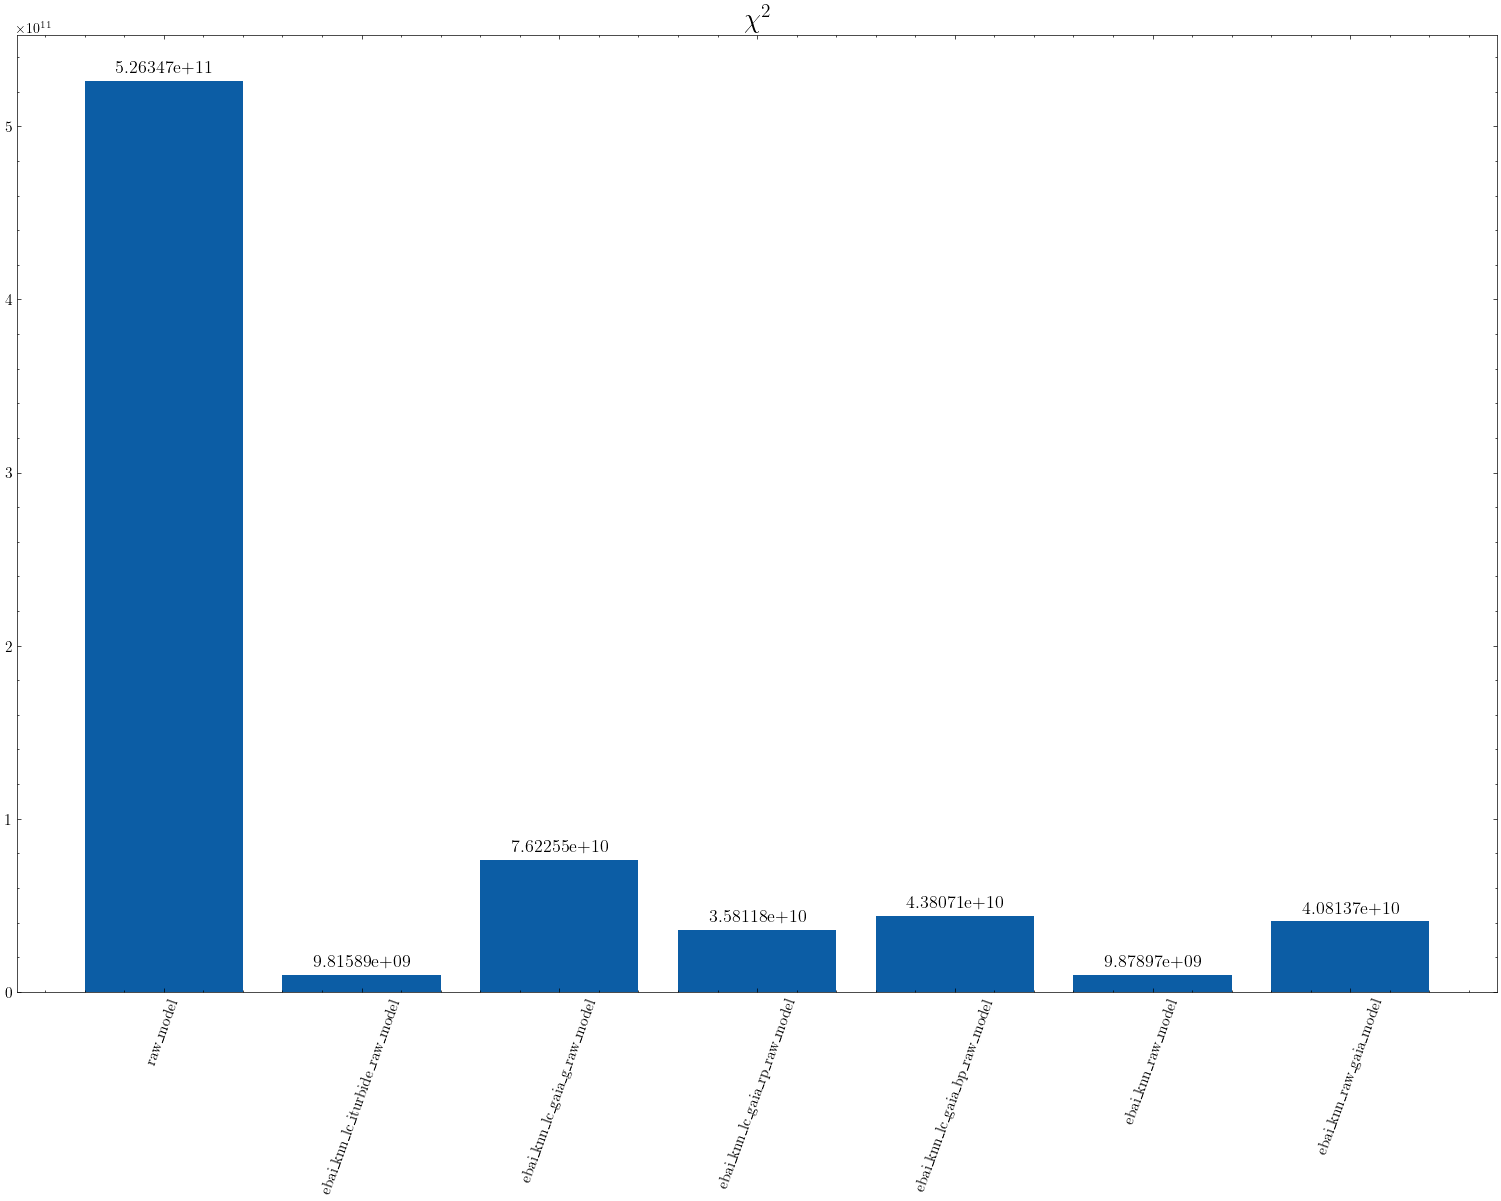
\includegraphics[scale=0.325]{Metodologia/Secciones/ModeloComputacional/Figures/EstimadoresChiResultados.png}
	\caption{Resultados del ajuste ($\lambda$) de los modelos sintéticos
		generados utilizando los parámetros dados por cada estimador. Cada
		estadística fue calculada con respecto a todos los datos observacionales
		disponibles, sin importar las combinaciones de curvas de luz utilizadas
		para hacer la estimación. \code{default\_model} corresponde al modelo
		inicial que ofrece PHOEBE a través de la función
		\code{phoebe.default\_contact\_binary()}. Los nombres de los estimadores
		en el eje vertical de la gráfica indican los datos observacionales
		utilizados para cada estimación de parámetros, junto al valor del ajuste
		el modelo sintético a todas las curvas del modelo. }
	\label{figuraEstimadoresLambda}
\end{figure}

\begin{figure}[!ht]
	\centering
	\xincludegraphics[scale=0.36]{Metodologia/Secciones/ModeloComputacional/Figures/ebaiKnnIturbideNorm.png}
	\xincludegraphics[scale=0.36]{Metodologia/Secciones/ModeloComputacional/Figures/ebaiKnnGaiaRaw.png}
	\xincludegraphics[scale=0.36]{Metodologia/Secciones/ModeloComputacional/Figures/ebaiKnnZtf.png}

	\caption{Modelos sintéticos del modelo utilizando los parámetros estimados
	por \code{ebai\_knn\_ztf\_gaia\_solver} junto a los residuos en los flujos
	para cada curva de luz. Estos modelos fueron sintetizados utilizando un
	factor de escala de flujos flexible, utilizando la opción \code{pblum\_mode
	= "dataset\_scaled"}, el cual nos permite analizar la morfología del modelo
	sintético sin considerar por ahora el efecto en la escala de la curva de
	parámetros relacionados con la luminosidad de cada componente, como las
	temperaturas absolutas o los radios de ambas estrellas. Estos parámetros son
	ajustados en los siguientes pasos de afinación del modelo.}
	\label{figuraEstimacionInicialModelo}
\end{figure}

\begin{table}[!ht]
	\centering
	\begin{tabular}{|l|l|}
		\hline
		% \rowcolor{blue}
		\thead{Parámetro}                        & \thead{Valor} \\
		\hline
		\code{t0\_supconj@binary}                & 0.02571 d    \\
		\hline
		\code{teffratio@binary}                  & 0.98746       \\
		\hline
		\code{incl@binary}                       & 70.3197 deg  \\
		\hline
		\code{fillout\_factor@contact\_envelope} & 0.25767       \\
		\hline
		\code{q@binary}                          & 1.93380       \\
		\hline
	\end{tabular}
	\caption{Resultados adoptados de las estimaciones iniciales, utilizando el
		estimador cuyos datos de entrada fueron las curvas de Gaia y ZTF. Las
		unidades de cada valor son especificadas excepto para los parámetros
		adimensionales.}
	\label{ebaiKnnInitialEstimationsValues}
\end{table}

\section{Optimización de Parámetros} \label{metodologia:modelocomputacional:optimizacion}

Como se puede ver en la \reffigure{figuraEstimacionInicialModelo} el modelo
inicial de PHOEBE no se ajusta perfectamente a los datos observacionales, esto
se aprecia mejor a partir de los residuos de cada curva de luz. En la siguiente
etapa del proyecto se emplea un muestreo MCMC, el cual en teoría es capaz de
determinar el mínimo global del espacio de parámetros, pero a un costo
computacional que crece exponencialmente con la distancia de los parámetros del
sistema actuales al mínimo global de la función de calidad.

El proceso de optimización de parámetros es distinto para cada sistema modelado;
ciertas estrategias pueden funcionar para un sistema y al mismo tiempo no llegar
a una solución adecuada para otro sistema. Para el caso de
\atoObjId primero se ajustó el tiempo de superconjunción; los
eclipses del modelo sintético están desfasados de los eclipses de las curvas
observadas en la \reffigure{figuraEstimacionInicialModelo}. Esto resultó en un
nuevo valor de $0.02589 \ \mathrm{d}$ para el tiempo de superconjunción. 
Utilizando un optimizador de Nelder Mead Simplex (\textit{NMS}, descrito en la
\refthesissubsubsection{intro:phoebe:nelder_mead}) se buscó optimizar los
parámetros configurados en la estimación inicial del modelo. Con la finalidad de
obtener un ajuste consistente y solo utilizar datos de alta calidad se decidió 
emplear las dos curvas de luz de ZTF para el resto del ajuste del modelo. Esto
se debe al número de datos; son más numerosas que
las observaciones hechas por Gaia, y son de mejor calidad que las realizadas
desde el OAU. Además al tener observaciones simultaneas en diferentes pasabandas
también es posible determinar las temperaturas efectivas de las componentes
estelares. 

El primer optimizador NMS corrigió la razón de temperaturas efectivas 
(el cual sirve para modificar la luminosidad relativa de la
estrella secundaria con respecto a la primaria, ajustando la profundidad del
eclipse secundario con respecto al eclipse primario), el factor de relleno
\code{fillout\_factor} (que sirve como una parametrización de la razón de radios
de las estrellas, ajustando el ancho de ambos eclipses), la inclinación orbital
del sistema \code{incl@binary} (que dicta el aspecto de los eclipses observados
con respecto al plano de observación, determinando la profundidad y la agudeza
de los eclipses), y la razón de masa \code{q}. La razón de masa no es un
parámetro que se pueda constreñir bien utilizando solo información fotométrica;
esto se debe a las correlaciones presentes en el modelo con los demás parámetros
del sistema. Después de 114 iteraciones el optimizador logró converger a una
solución mostrada en la \reftable{tablaOptNmResultados}.

\begin{table}[!ht]
	\centering
	\begin{tabular}{|l|l|}
		\hline
		\thead{Parámetro}                        & \thead{Valor optimizado} \\
		\hline
		\code{teffratio@binary}                  & 1.07991       \\
		\hline
		\code{incl@binary}                       & 70.19810 deg  \\
		\hline
		\code{fillout\_factor@contact\_envelope} & 0.09356       \\
		\hline
		\code{q@binary}                          & 2.13478       \\
		\hline
	\end{tabular}
	\caption{Valores optimizados utilizando el algoritmo Nelder-Mead Simplex.}
	\label{tablaOptNmResultados}
\end{table}

\begin{figure}
	\centering
	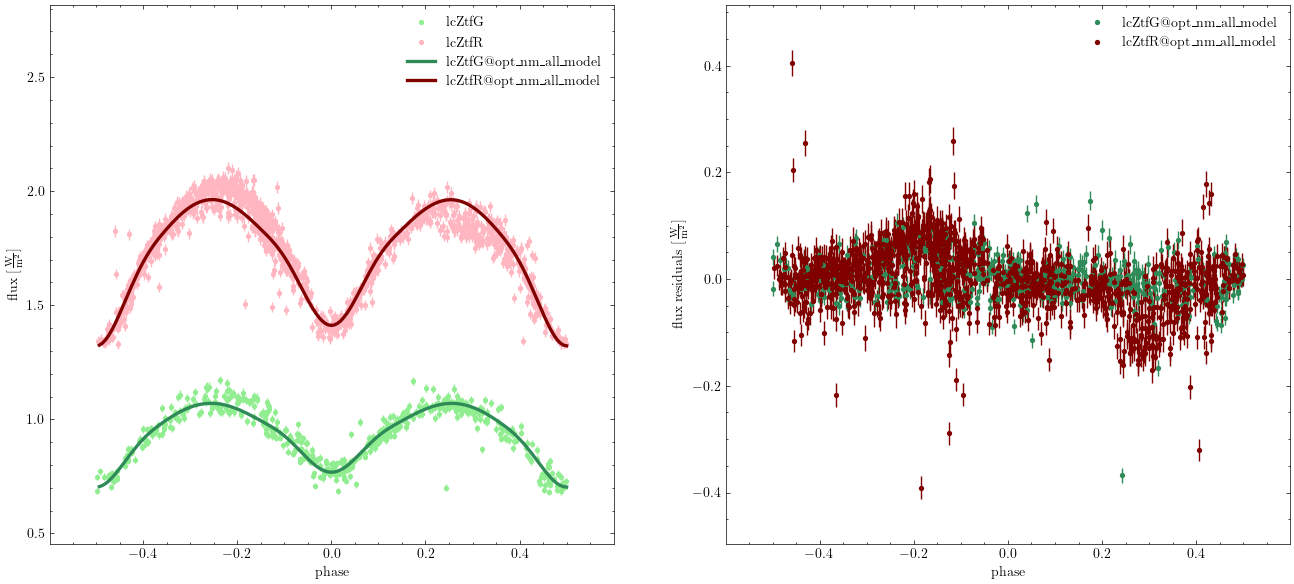
\includegraphics[scale=0.44]{Metodologia/Secciones/ModeloComputacional/Figures/Figura Opt NM Resultados ZTF.png}
	\caption{Modelo sintético generado utilizando los parámetros dados por el
	optimizador NMS, vistos en la \reftable{tablaOptNmResultados}, utilizando el
	tiempo de superconjunción corregido.}
	\label{figuraOptNmResultadosZtf}
\end{figure}

La curva sintética del modelo optimizado visto en la
\reffigure{figuraOptNmResultadosZtf} muestra una asimetría en las jorobas de la
curva de luz en fase. Estos máximos corresponden a las fases orbitales en las
cuales la mayor cantidad de elementos superficiales de ambas componentes
coinciden con nuestra línea de observación. Este fenómeno se le denomina el
\textit{efecto O'Connell}, descrito originalmente por
\citeyearparen{oconnell_periastron_effect-OConnell_effect_1951} donde se
distingue del efecto de periastro que es causado por efectos de marea en
sistemas con órbitas excéntricas. El \textit{efecto O'Connell} se debe a la
diferencia de luminosidad entre diferentes hemisferios de una estrella; puede
ser causado por un punto caliente debido a la acreción de material en el caso de
haber una alta tasa de transferencia de masa
(\citeyearparen{darwish_light_curve_analysis_four_new_short_period_eclipsing_binaries_2024}),
o por manchas en la superficie estelar debido a actividad en la fotósfera. Para
llegar a un mejor ajuste de la curva fotométrica se introdujo una mancha fría en
la estrella secundaria. Después de hacer un ajuste manual de los parámetros de
la mancha se utilizó un optimizador NMS para obtener los parámetros óptimos de
la mancha estelar. Los parámetros optimizados se pueden ver en la
\reftable{tablaOptManchaResultados}, y la mancha estelar se puede ver
representada en la \reffigure{figuraMallaManchaNm}.

% TODO: style table
\begin{table}[!ht]
	\centering
	\begin{tabular}{|l|l|}
		\hline
		% \rowcolor{blue}
		\thead{Parámetro}	& \thead{Valor optimizado} \\
		\hline
		\code{colat}	& 89.77983 deg	\\
		\hline
		\code{long}		& 81.09966 deg  \\
		\hline
		\code{radius} 	& 25.12086 deg	\\
		\hline
		\code{relteff}	& 0.93007		\\
		\hline
	\end{tabular}
	\caption{Parámetros de la mancha estelar optimizados utilizando el algoritmo
	Nelder-Mead Simplex, el cual logró converger después de 102 iteraciones.
	Todos los parámetros son relativos a la superficie estelar a la que le
	pertenece la mancha; la longitud \code{long} donde se define la longitud
	$0^{\circ}$ viendo a la estrella primaria, la latitud \code{colat} se define
	como el ángulo polar empezando desde el polo norte de la estrella, el radio
	angular \code{radius}, y la temperatura efectiva relativa \code{relteff} con
	respecto a la temperatura superficial.}
	\label{tablaOptManchaResultados}
\end{table}

\begin{figure}[!ht]
	\centering
	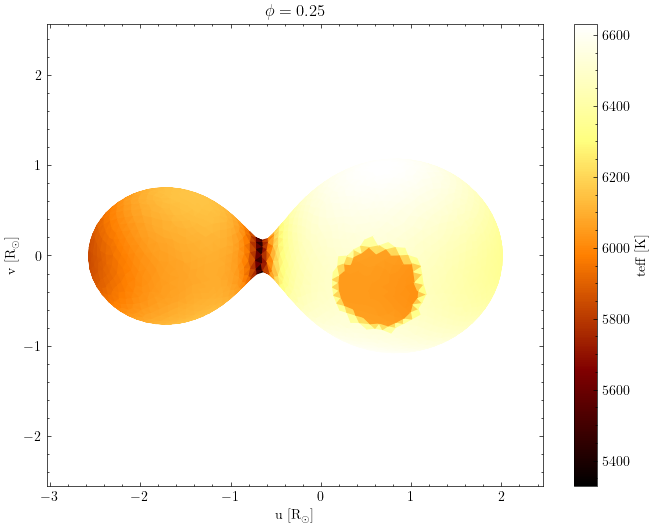
\includegraphics[scale=0.8]{Metodologia/Secciones/ModeloComputacional/Figures/Figura Malla Mancha NM.png}
	\caption{Malla representando la superficie estelar de ambas componentes en
	su fase orbital $\phi = 0.25$, en el máximo menor de la curva fotométrica.
	Aquí se puede apreciar la mancha estelar introducida a la componente
	secundaria. La temperatura efectiva de cada elemento superficial de la
	envoltura en común, donde la mancha se ve de un color más oscuro debido a su
	baja temperatura con respecto al resto de la superficie estelar.}
	\label{figuraMallaManchaNm}
\end{figure}

Una vez que se logró un nivel de ajuste adecuado con los optimizadores
de tipo NMS se aplicó un último ajuste utilizando correcciones diferenciales,
los cuales funcionan mejor cuando los parámetros se encuentren lo
suficientemente cerca del mínimo global, para evitar caer y estar atrapados
dentro de un mínimo local. El motivo para acercarnos lo más posible al mínimo
global es para reducir el trabajo del muestreo MCMC; entre mayor sea la
distancia que los caminadores tengan que recorrer, se requerirá más iteraciones
para obtener un muestreo adecuado del espacio de parámetros. El resolvedor se
crea con el código en la \refcode{codigoOptimizadorDc}, en donde se define el
tamaño de los pasos que intenta hacer el optimizador; estos deben de ser
suficientemente pequeños para evitar saltos fuera del área de interés, pero
suficientemente grandes para que haya un cambio en el ajuste del modelo. El
tamaño de los pasos se determinó por medio de experimentación manual del efecto
en un modelo sintético de PHOEBE.

\begin{figure}[!ht]
	\begin{lstlisting}[language=Python, autogobble]
		b.add_solver('optimizer.differential_corrections', solver='dc_relative', overwrite=True,
             fit_parameters=['teffratio', 'incl@binary', 'fillout_factor', 'q'],
             steps={
                'q': 0.01,
                'incl@binary': 1,
                'fillout_factor': 0.01,
                'teffratio': 0.01
             })
	\end{lstlisting}
	\caption{Código que se utilizó para crear el optimizador de correcciones
	diferenciales para los parámetros que dictan la forma de la curva de luz en
	fase. El argumento \code{steps} del optimizador representa $\Delta
	\mathbf{p} = \{ \Delta p_1, ..., \Delta p_k \}$ visto en la
	\refequation{ecuacionDiferenciasFinitas}.}
	\label{codigoOptimizadorDc}
\end{figure}

\begin{table}[!ht]
	\centering
	\begin{tabular}{|l|l|}
		\hline
		\thead{Parámetro}                        & \thead{Valor optimizado} \\
		\hline
		\code{teffratio@binary}                  & 1.06676       \\
		\hline
		\code{incl@binary}                       & 68.42157 deg  \\
		\hline
		\code{fillout\_factor@contact\_envelope} & 0.07892       \\
		\hline
		\code{q@binary}                          & 1.10457       \\
		\hline
	\end{tabular}
	\caption{Valores optimizados utilizando un optimizador de correcciones diferenciales.}
	\label{tablaOptDcResultados}
\end{table}

Después de 17 iteraciones se obtuvieron los parámetros vistos en la
\reftable{tablaOptDcResultados}, de los cuales se generaron las curvas sintéticas
vistas en la \reffigure{figuraOptDcResultadosZtf}. El optimizador de
correcciones diferenciales no se utilizó para ajustar los parámetros de la
mancha estelar; estos se mantuvieron fijos en sus valores determinados por el
optimizador NMS para después explorar utilizando MCMC.

\begin{figure}[!ht]
	\centering
	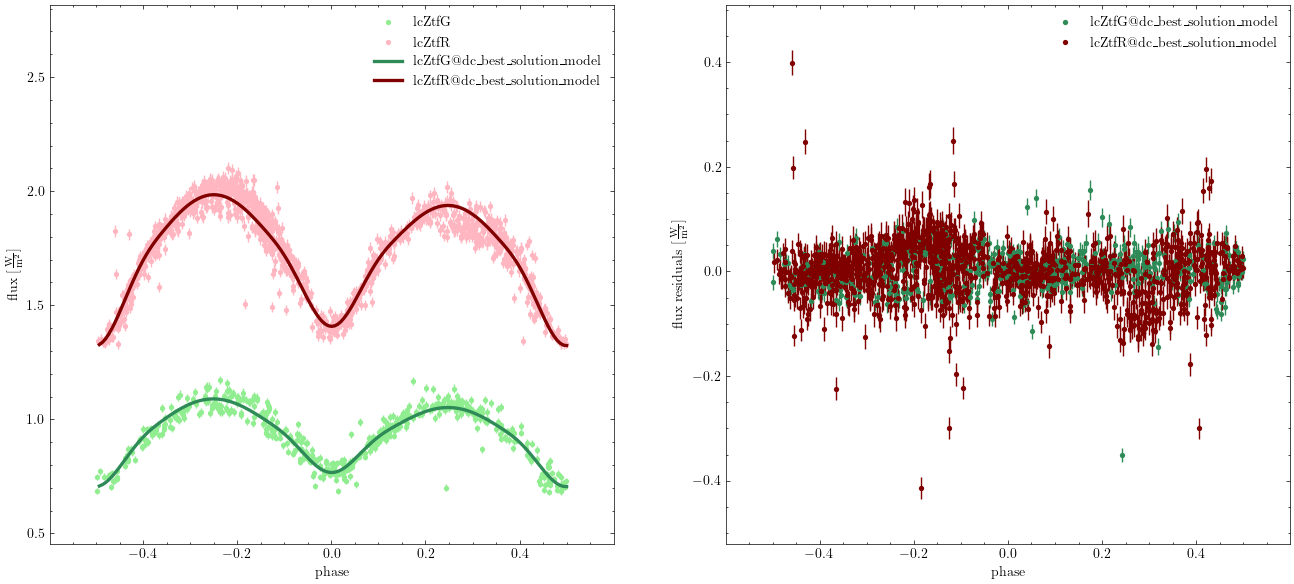
\includegraphics[scale=0.45]{Metodologia/Secciones/ModeloComputacional/Figures/Figura Opt DC Resultados ZTF.png}
	\caption{Modelo sintético junto a el residuo de flujo tomando en cuenta una
	mancha estelar fría en la componente secundaria (vista en la
	\reffigure{figuraMallaManchaNm}) y utilizando los parámetros resultados del
	proceso de optimización vistos en la \reftable{tablaOptDcResultados}.}
	\label{figuraOptDcResultadosZtf}
\end{figure}

\section{Ajuste de Luminosidad y Temperatura Efectiva} \label{metodologia:modelocomputacional:ajuste_luminosidad_teff}

Utilizando las curvas calibradas de ZTF en ambas pasabandas se determinó la
temperatura efectiva del sistema partiendo unicamente de las curvas
fotométricas. Para esto se manipularon en total 3 parámetros del sistema: la
temperatura efectiva de la componente primaria (\code{teff@primary}), la razón
de temperaturas de las componentes $T_2 / T_1$ (\code{teffratio}), y el factor
de escala de la luminosidad de pasabanda (\code{pblum@primary@lcZtfG}) para la
pasabanda ZTF:g. Se acopló la temperatura efectiva del sistema al color (dado
por el flujo relativo entre las curvas de ZTF) utilizando el modo
\code{pblum\_mode} con el valor \code{component-coupled} para la curva de ZTF:g,
y un valor de \code{dataset-coupled} para la curva de ZTF:r. En el modo
\code{component-coupled} el usuario proporciona un valor para la luminosidad
emergente de la componente primaria en el tiempo $t_0$ del sistema, a partir del
cual PHOEBE determina un factor de escala tal que las intensidades superficiales
de las estrellas sean igual a la luminosidad dada. El modo
\code{dataset-coupled} aplica el mismo factor de escala a la curva de ZTF:r que
el factor dado a la curva ZTF:g, manteniendo información del color del sistema
(\citeyearparen{conroy_phoebe_v_framework_solving_inverse_problem_2020}). 

Una vez que se haya establecido esta configuración del bundle se aplicó un
optimizador de tipo NMS para ajustar los tres parámetros mencionados en el
párrafo pasado. Como valor inicial se ajustó manualmente la temperatura efectiva
de la primaria a $4600 \ \mathrm{K}$, el cual se determinó por medio de
experimentación manual. Después de 174 iteraciones el optimizador logró
converger a la solución dada en la \reftable{tablaOptNmTeffResultados}. Dado que
estos parámetros principalmente afectan el factor de escala de las curvas de
luz, los demás parámetros del sistema se mantuvieron fijos, manteniendo la forma
de las curvas de luz.

\begin{table}[!ht]
	\centering
	\begin{tabular}{|l|l|}
		\hline
		\thead{Parámetro}                        & \thead{Valor optimizado} \\
		\hline
		\code{teff@primary}							& 4203.69115 K  \\
		\hline
		\code{teffratio@binary}						& 1.05213       \\
		\hline
		\code{pblum@primary@lcZtfG}					& 4.78643 W       \\
		\hline
	\end{tabular}
	\caption{Valores optimizados para la temperatura efectiva de la estrella
	primaria, junto a la luminosidad de pasabanda que produce el factor de
	escala necesario para ajustar a la curva fotométrica. La temperatura
	efectiva de la secundaria está constreñida por la temperatura efectiva de la
	primaria y la razón de temperaturas; dado estos parámetros, la temperatura
	efectiva secundaria es igual a 4422.837561158592 K.}
	\label{tablaOptNmTeffResultados}
\end{table}

\section{Muestreo MCMC} \label{metodologia:modelocomputacional:mcmc}

Una vez que obtuvimos el conjunto de parámetros que mejor ajustan el
modelo sintético a los datos observacionales buscamos obtener las incertidumbres
para cada parámetro. La manera recomendada por el equipo de desarrollo de PHOEBE
es por medio de un muestreo Bayesiano \textit{Monte Carlo Markov Chain}.
Utilizando un muestreo MCMC es posible determinar la morfología del espacio de
parámetros de manera holística; esto permite identificar cualquier correlación
que exista entre los parámetros del sistema. El proceso de muestreo empleado en
este proyecto es por PHOEBE utilizando el paquete de Python \code{emcee},
descrito en la \refthesissubsection{intro:phoebe:problema_inverso:muestreo}.
Antes de correr el proceso de muestreo se preparó el bundle de la siguiente
manera.

\subsection{Eliminación de Observaciones Erróneas} \label{metodologia:modelocomputacional:mcmc:eliminacion_errores}

PHOEBE utiliza la probabilidad logarítmica ($\mathrm{lnprobability}$) del modelo
sintético como la \textit{función de mérito} para el muestreo. Esta se define en
la siguiente ecuación:

\begin{eqfloat}[!ht]
	\centering
	\begin{equation}
		\textrm{lnprobability} = \textrm{lnpriors} + \textrm{lnlikelihood}
	\end{equation}
\end{eqfloat}

Donde $\mathrm{lnpriors} = \sum_{\Pi} \ln{P(p | \pi)}$ es la probabilidad
logarítmica de obtener los parámetros actuales del modelo $p$ de una
distribución a priori $\pi$ sumando sobre todas las distribuciones priores $\Pi$
(\citeyearparen{conroy_phoebe_v_framework_solving_inverse_problem_2020}). El
término $\mathrm{lnlikelihood}$ es la verosimilitud, la cual está definida en
la \refequation{ecuacionLnLikelihoodMcmc}. Tras varios experimentos corriendo
varias instancias del muestreo MCMC se descubrió que los caminadores son
excepcionalmente sensibles a fluctuaciones en la función de mérito; las
observaciones que se desvían de manera significativa de la región principal de
la curva de luz en fase indican un ajuste inadecuado según la función de mérito.
Debido a que las incertidumbres de estos puntos probablemente fueron registradas
de manera errónea estos puntos se eliminaron de la curva observada. En el
Notebook
\href{https://github.com/KnightIV/UANL_MAPTA_Observaciones/blob/main/analisis/phoebe_model/sampling/remove-bad-observations.ipynb}{\code{remove-bad-observations.ipynb}}
se aplicó un criterio a la desviación estándar de los residuos del modelo
optimizado; aquellos puntos cuya diferencia con el modelo sintético sea mayor de
un múltiplo de la desviación estándar fue eliminado de los datos. Los resultados
de esta optimización se pueden ver en la
\reffigure{figuraEliminarMalasObservacionesZtf}. El modelo sintético utilizando
solo estos datos se puede ver en la
\reffigure{figuraModeloSinMalasObservacionesZtf}, donde se puede apreciar a
mayor detalle la forma oscilatoria de los residuos. Esto indica que los valores
obtenidos no son los óptimos y aún hay más cambios que se podrían emplear para
llegar a un mejor ajuste; sin embargo, este es un ajuste suficientemente bueno
para este proyecto para continuar al muestreo del espacio de parámetros con
MCMC.

\begin{figure}[!ht]
	\centering
	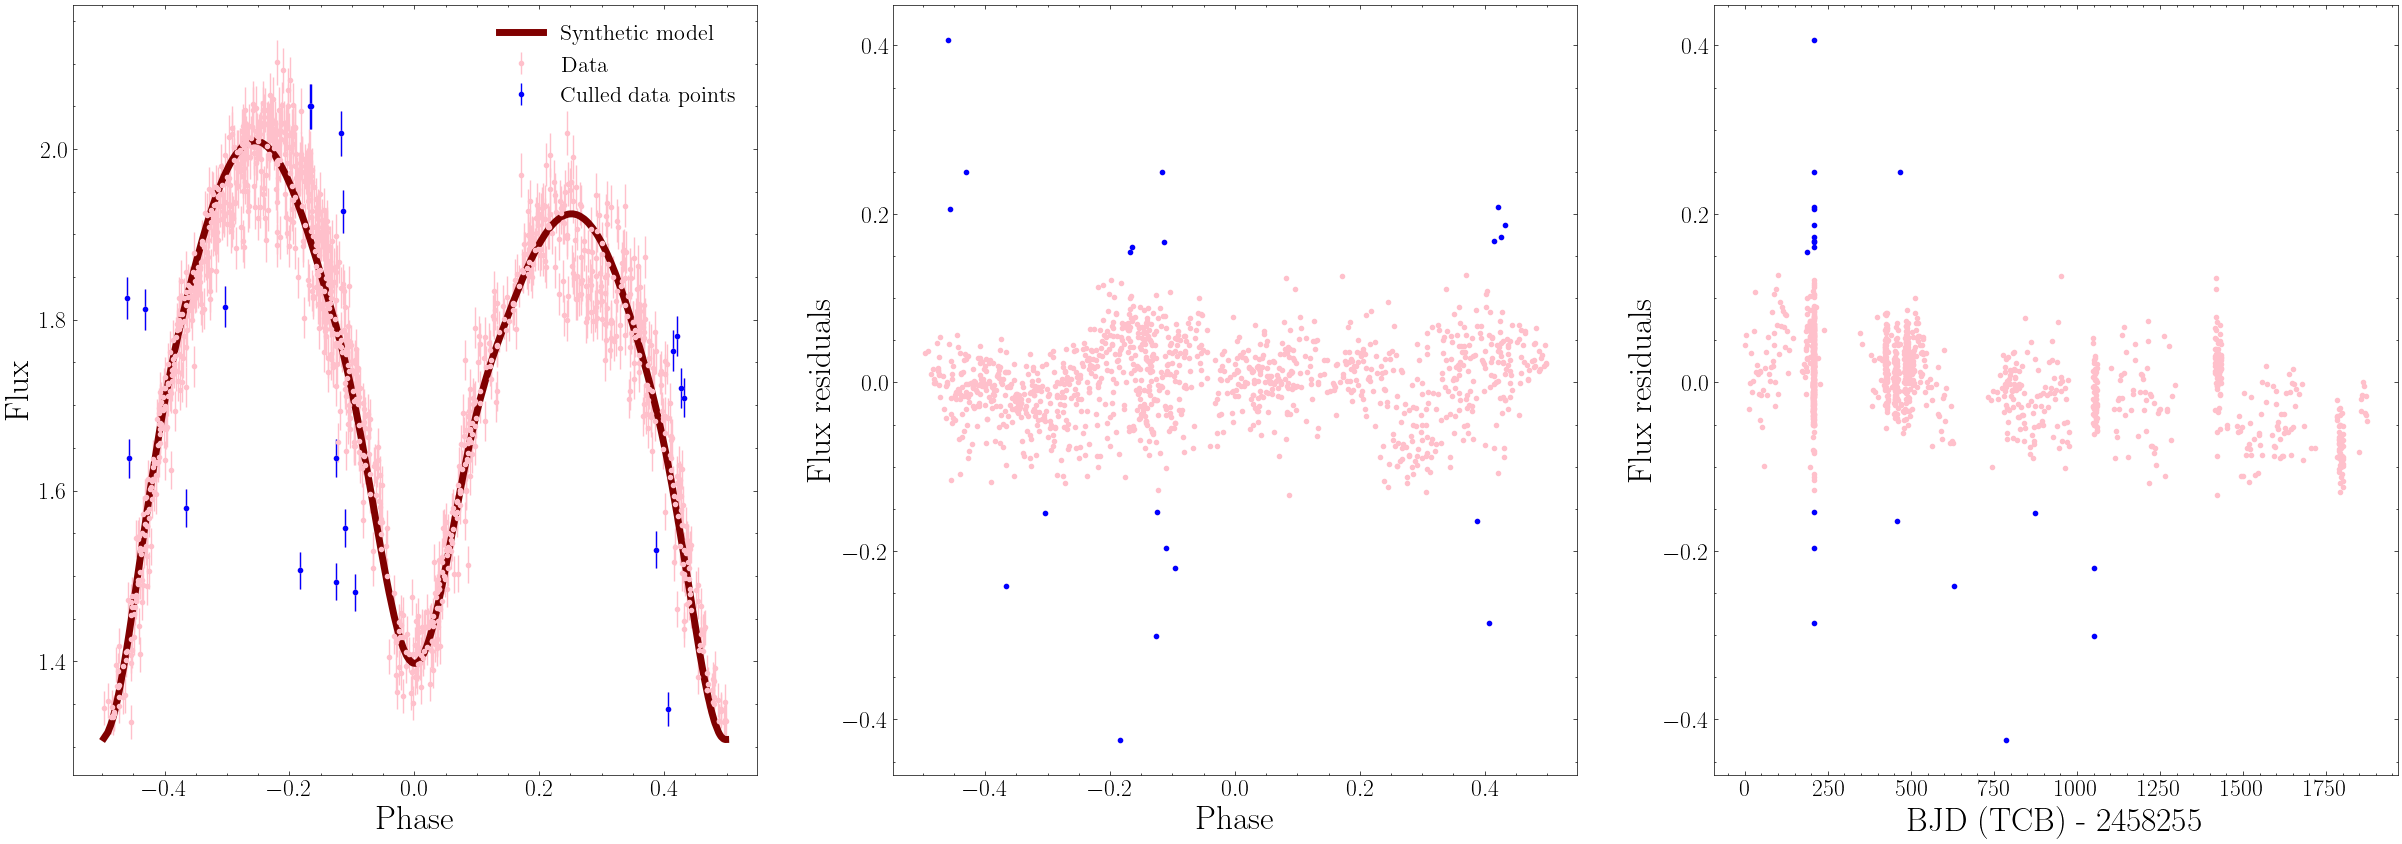
\includegraphics[scale=0.24]{Metodologia/Secciones/ModeloComputacional/Figures/Figura Malas Observaciones ZTF:r.png}
	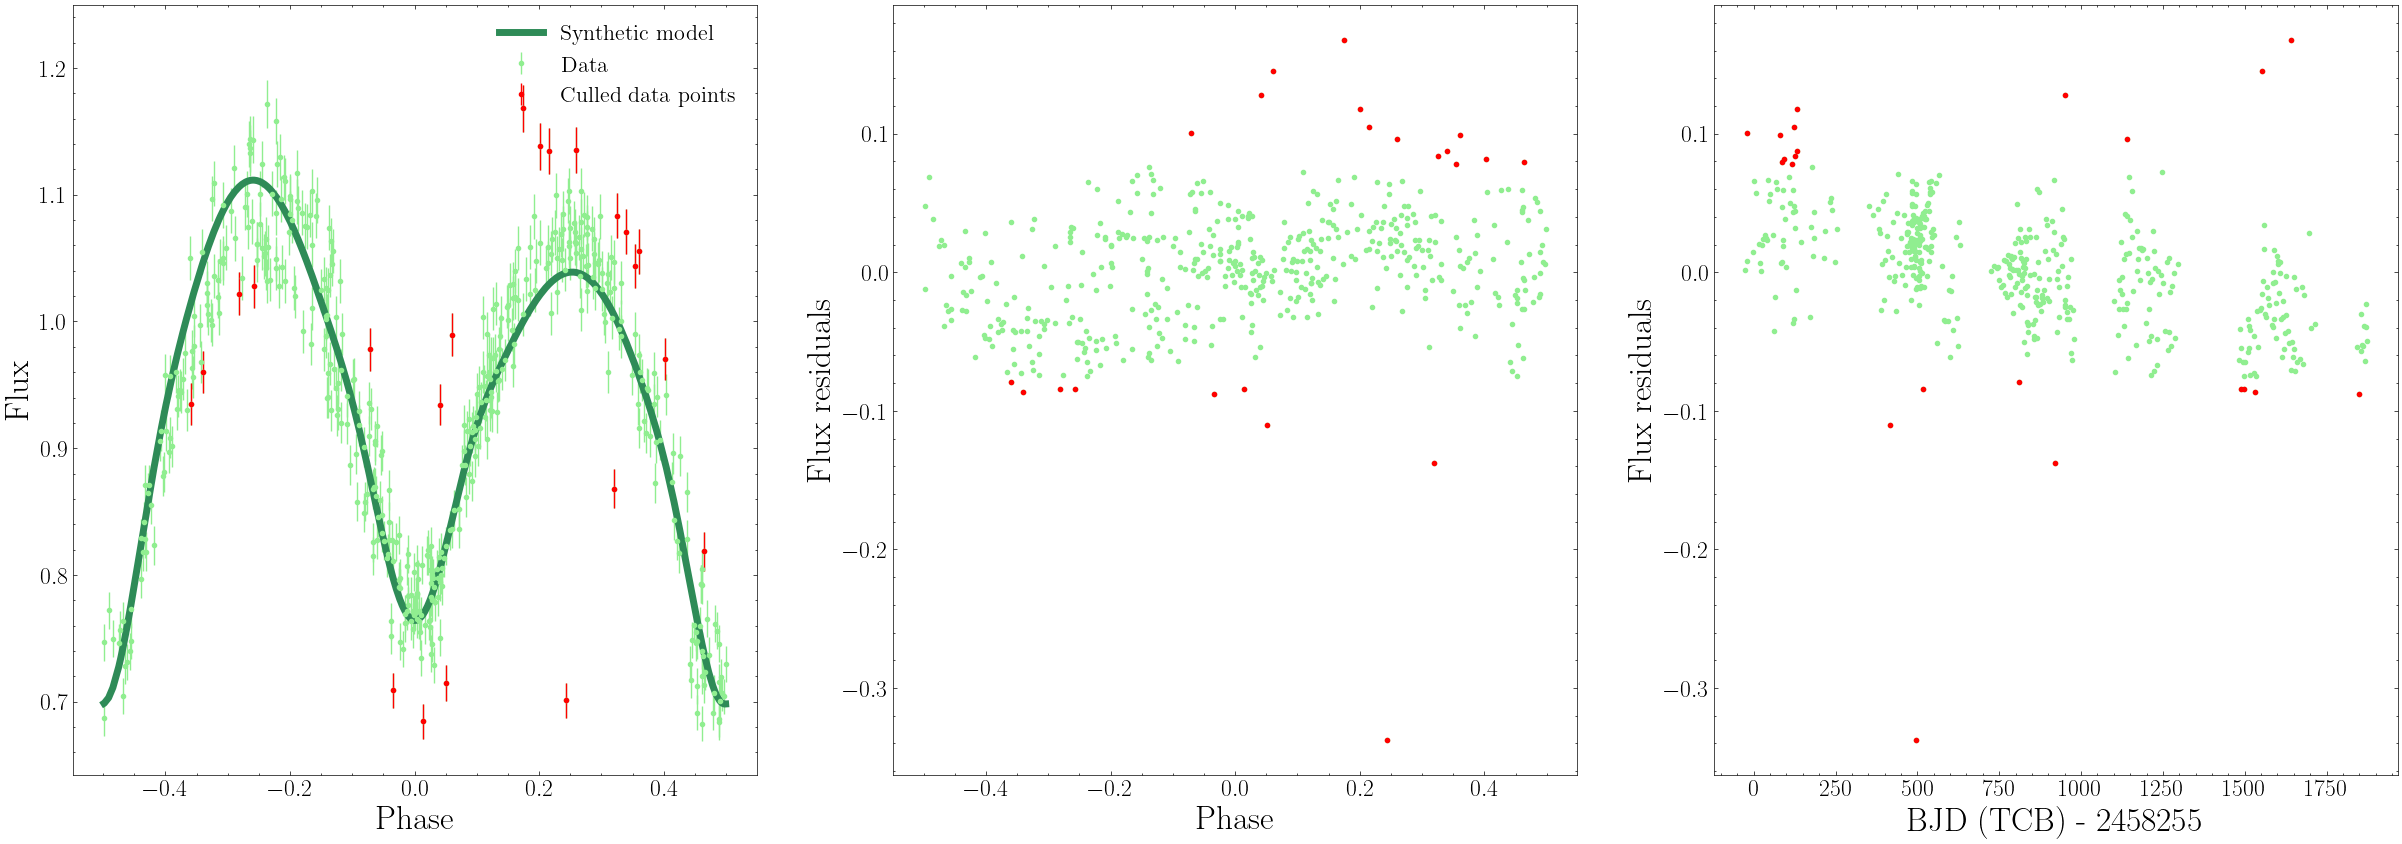
\includegraphics[scale=0.24]{Metodologia/Secciones/ModeloComputacional/Figures/Figura Malas Observaciones ZTF:g.png}
	\caption{Resultados de aplicar el criterio de eliminación para las curvas de
	luz de ZTF, donde la figura superior corresponde a el pasabanda ZTF:r y la
	inferior a ZTF:g. Se optó por codificar este criterio en el código en vez de
	eliminar los datos manualmente para ser fácilmente reproducible. El factor
	de escala del criterio fue ajustado manualmente tal que los puntos más
	erróneos sean eliminados con éxito, y al mismo tiempo preservar la forma y
	dispersión principal que existen en los datos.}
	\label{figuraEliminarMalasObservacionesZtf}
\end{figure}

\begin{figure}[!ht]
	\centering
	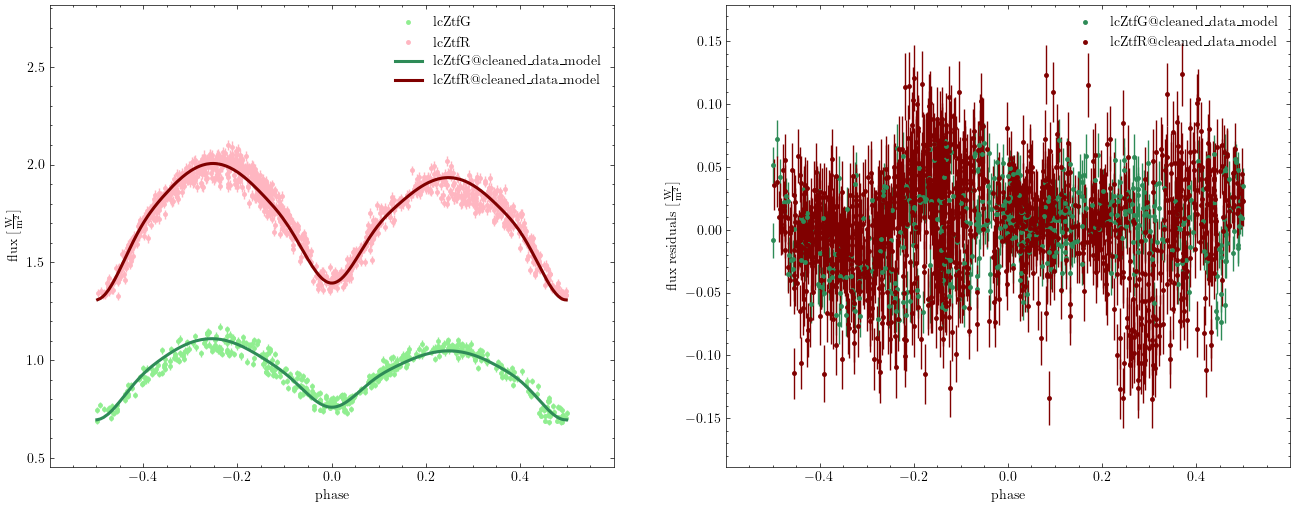
\includegraphics[scale=0.44]{Metodologia/Secciones/ModeloComputacional/Figures/Figura Modelo Sin Malas Observaciones ZTF.png}
	\caption{Modelo sintético en las pasabandas de ZTF calculado después de
	eliminar las observaciones más problemáticas de las curvas observadas.}
	\label{figuraModeloSinMalasObservacionesZtf}
\end{figure}

\subsection{Distribuciones Priores}

Para poder muestrear el espacio de parámetros, el algoritmo MCMC requiere de una
región inicial a partir de cual inicializar las posiciones de cada caminador.
Estas distribuciones iniciales también actúan como una guía; al principio del
muestreo los caminadores en su mayoría no saldrán de las regiones de
concentración de estas distribuciones. La forma de las priores dejará de
importar entre más iteraciones logre correr la cadena, de la cual se
estimará la distribución posterior de densidad de cada parámetro.

PHOEBE ofrece unas herramientas para los tipos de distribuciones más comunes en
este trabajo: la distribución uniforme y la distribución Gaussiana (normal).
Para el muestreo de \atoObjId se utilizaron distribuciones uniformes para los
parámetros ajustables del bundle\textemdash todos aquellos que han sido
ajustados a lo largo de la optimización de parámetros. Una distribución uniforme
no tiene un significado físico intrínseco más allá de comunicar una falta de
información del problema. En nuestro caso, las priores sirven para marcar un
límite práctico para cada parámetro, tanto para evitar que los caminadores se
pierdan en espacios que produzcan un resultado no físico, cómo para constreñir
el volumen de interés a lo más cercano de los parámetros óptimos derivados en el
proceso de optimización. 

Se crearon tres colecciones de distribuciones en el bundle de PHOEBE para
delimitar los parámetros ajustables del modelo: uno para los parámetros de
interés del sistema binario, otro para los parámetros que rigen la mancha
estelar en la componente secundaria, y finalmente uno que restringe el factor de
escala en el pasabanda ZTF:g. Las colecciones individuales de distribuciones
priores se pueden ver en la \reffigure{figuraColeccionesPrioresZtf}, la
\refthesissection{apendice:modelo_computacional_graficas:dist_priores_completas}
muestra todos los priores utilizados para el proceso de MCMC.

\begin{figure}[!ht]
	\centering
	\xincludegraphics[scale=0.25, label=\textbf{(a)}, labelbox=true, pos=ne, fontsize=\Large]{Metodologia/Secciones/ModeloComputacional/Figures/Figura Prior Params Binaria.png}
	\xincludegraphics[scale=0.32, label=\textbf{(b)}, labelbox=true, pos=ne, fontsize=\Large]{Metodologia/Secciones/ModeloComputacional/Figures/Figura Prior Params Mancha.png}
	\xincludegraphics[scale=0.77, label=\textbf{(c)}, labelbox=true, pos=ne, fontsize=\Large]{Metodologia/Secciones/ModeloComputacional/Figures/Figura Prior Params Luminosidad ZTF.png}
	\caption{Distribuciones priores utilizadas como límites iniciales a cada
	caminador. Se separaron en 3 distintas colecciones por cuestiones de
	organización dentro del código: \textbf{(a)} los parámetros principales del
	sistema solar que afectan la forma de la curva fotométrica sintética en
	orden de izquierda a derecha y de arriba a abajo: la temperatura efectiva de
	la componente primaria ($T_{1}$), la razón de temperaturas ($T_2/T_1$), el
	factor de relleno ($f$), la inclinación orbital ($i_{\mathrm{orb}}$), y la
	razón de masas ($q$). \textbf{(b)} los parámetros de la mancha estelar en la
	componente secundaria que se introdujo para tomar en cuenta el efecto
	O'Connell: su posición con respecto al origen del sistema de coordenadas en
	la secundaria (su longitud y latitud), el radio angular, y la
	razón de temperatura de la mancha a la temperatura efectiva
	de la superficie estelar. \textbf{(c)} la
	luminosidad en el pasabanda ZTF:g, la cual determina el factor de escala de
	las curvas de luz de ZTF.}
	\label{figuraColeccionesPrioresZtf}
\end{figure}

% TODO: formatting new page
\newpage
\clearpage

\subsection{Inicializando el Muestreo MCMC}

Una vez que se determinaron las distribuciones priores a utilizar para
inicializar la cadena se pudo empezar el muestreo. Se emplearon 160 caminadores
en total; en general, es mejor tener la mayor cantidad de caminadores posible
tal que sea mayor que la cantidad de parámetros que se van a explorar (10
parámetros vs. 160 caminadores). Esto también está restringido por el cómputo
disponible. El algoritmo \textit{stretch-move} descrito por
\citeyearparen{foreman-mackey_emcee_2013} muestra que un ensamble no es
completamente paralelizable, por lo tanto no es necesario restringir la cantidad
de caminadores estrictamente al número de procesadores (hilos) disponibles en
una computadora. 

El muestreo MCMC se corrió en un servidor propiedad del Dr. Carlos Esteban
Chávez Pech de la Facultad de Ingeniería Mecánica y Eléctrica en la Universidad
Autónoma de Nuevo León. Este servidor cuenta con 4 CPUs físicos AMD Opteron(tm)
Processor 6376, el cual suma a 64 procesadores virtuales disponibles al sistema
operativo (y por ende al código MCMC). La computadora está equipada con 32 GB de
memoria RAM\textemdash a pesar que el mayor costo del muestreo es en el cómputo
directo, la cantidad de memoria requerida aumenta rápidamente entre más
caminadores se utilizan debido a la copia de datos necesaria por el proceso de
paralelización por medio del módulo \code{multiprocessing} de Python. El
muestreo final de este trabajo utilizó 13 GB de memoria, el cual fue asignado
por el código al principio del proceso, manteniéndose estable por el resto del
tiempo de cómputo.

Para poder estar revisando el progreso del muestreo se configuró el resolvedor
para guardar su cadena actual cada 5 iteraciones. Cada iteración en
promedio tardó entre 520 a 560 segundos por terminar, lo cual resultaba en un
reporte de progreso aproximadamente cada 45 minutos. Esto también actúa como
un respaldo; si el proceso termina de manera errónea es posible reiniciar el
muestreo partiendo de la última iteración registrada en el archivo de progreso. 

\subsection{Monitoreo del Muestreo}

\subsubsection{Tiempo de Autocorrelación}

Un proceso de MCMC se puede considerar finalizado una vez que los caminadores
hayan convergido a una región particular en el espacio de parámetros. Debido al
proceso estocástico que cada caminador emplea para determinar su camino por el
espacio de parámetros, es esperado\textemdash y deseado\textemdash que en algún
momento vuelva a navegar el mismo camino que recorrió en iteraciones pasadas.
Cada nuevo conjunto de parámetros $\mathbf{\Theta}_i$ en una cadena
$\left\{\mathbf{\Theta}_1 \rightarrow ... \rightarrow \mathbf{\Theta}_i
\rightarrow ... \rightarrow \mathbf{\Theta}_n \right\}$ tiene una mayor
probabilidad de estar correlacionado con las posiciones previas
$\mathbf{\Theta}_{i - 1}$. Esto no es deseado, debido a que tener varias
muestras correlacionadas nos impide obtener una estimación adecuada de la
distribución posterior (\citeyearparen{speagle_conceptual_intro_mcmc_2020}).
Para determinar el grado de correlación entre cada paso en la cadena se utiliza
el \textbf{tiempo de autocorrelación} (\textbf{autocorrelation time} en inglés),
el cual se mide por medio de la autocovarianza que muestra la cadena utilizando
un desfase $t$.

\begin{eqfloat}[!ht]
	\begin{equation}
		C_f(t) = \lim_{n \rightarrow \infty} \left[\frac{1}{n} \sum_{i=1}^{n}{(\mathbf{\Theta}_i - \bar{\mathbf{\Theta}}) \cdot (\mathbf{\Theta}_{i+t} - \bar{\mathbf{\Theta}})}\right]
	\end{equation}
	\blankcaption
	\label{ecuacionAutocovarianza}
\end{eqfloat}

Utilizando la \refequation{ecuacionAutocovarianza} se calcula la covarianza
entre el vector de parámetros $\mathbf{\Theta}_i$ para la iteración $i$ y el
valor de la cadena después de $t$ iteraciones. El valor de $C_f(t)$ es mayor
cuando $t = 0$; cada valor está directamente correlacionado con sí mismo al ser
idénticos. De lo contrario, el valor teórico mínimo ocurre cuando los parámetros
obtenidos en la iteración $i$ e $i+t$ son completamente independientes. Se
define una función de autocorrelación $A(t)$ para un desfase $t$:

\begin{eqfloat}[!ht]
	\begin{equation}
		A(t) \equiv \frac{C_f(t)}{C_f(0)}
	\end{equation}
\end{eqfloat}

Del cual se define el \textbf{tiempo de autocorrelación integrado} $\tau_f$
por \citeyearparen{foreman-mackey_emcee_2013}:

\begin{eqfloat}[!ht]
	\begin{equation}
		\tau_f \equiv \sum_{t = -\infty}^{\infty} A(t) - 1 = \sum_{t = -\infty}^{\infty} \frac{C_f(t)}{C_f(0)} - 1 = 2 \sum_{t = 1}^{\infty} A(t)
	\end{equation}
	\blankcaption
	\label{ecuacionAutocorrIntegrado}
\end{eqfloat}

El término $-1$ se introduce para restar el caso de $A(0) = 1$. La integración
se restringe solo para $t > 0$; se multiplica por 2 debido a la simetría $A(t) =
A(-t)$ (\citeyearparen{speagle_conceptual_intro_mcmc_2020}). 

Dentro de PHOEBE existen funciones para calcular $\tau_f$ para cada parámetro en
la muestra; por lo tanto, la \refequation{ecuacionAutocovarianza} sería evaluada
para un parámetro a la vez, dándonos el número de iteraciones requeridas para
obtener muestras independientes de cada parámetro. En el código
\href{https://github.com/KnightIV/UANL_MAPTA_Observaciones/blob/main/analisis/phoebe_model/sampling/mcmc_utils.py}{\code{mcmc\_utils.py}}
se define la función \code{printParameterAutocorrTimes}, la cual imprime el
tiempo de autocorrelación de cada parámetro dada una cadena MCMC en la forma de
una solución. Un ejemplo se puede ver en la
\reffigure{codigoParamAutoCorrSalida}.

% TODO: replace with final solution
\begin{figure}[!ht]
	\centering
\begin{lstlisting}
Parameter autocorrelation times 
	Total iterations: 465 (131 burnin) 
	Avg. autocorr time: 47.22028105437427 
	Avg. IIDs: 7.073231936408811
---------------------------------------------------------------
teff@primary@star@component
	Autocorrelation time: 31.434501067709036
	IIDs ([iters - burnin]/autocorr_time): 10.625268054376729
teffratio@binary@orbit@component
	Autocorrelation time: 21.366271511782326
	IIDs ([iters - burnin]/autocorr_time): 15.632114373151971
fillout_factor@contact_envelope@envelope@component
	Autocorrelation time: 54.501126163049854
	IIDs ([iters - burnin]/autocorr_time): 6.128313734303019
incl@binary@orbit@component
	Autocorrelation time: 29.773153661983663
	IIDs ([iters - burnin]/autocorr_time): 11.218159950132302
q@binary@orbit@component
	Autocorrelation time: 65.7180243303593
	IIDs ([iters - burnin]/autocorr_time): 5.082319552410896
pblum@primary@lcZtfG@lc@dataset
	Autocorrelation time: 65.32641769723654
	IIDs ([iters - burnin]/autocorr_time): 5.1127860944092305
colat@secondary_spot@secondary@spot@feature
	Autocorrelation time: 64.5003963|1717
	IIDs ([iters - burnin]/autocorr_time): 5.178262756629427
long@secondary_spot@secondary@spot@feature
	Autocorrelation time: 38.025785518192954
	IIDs ([iters - burnin]/autocorr_time): 8.783513488240814
radius@secondary_spot@secondary@spot@feature
	Autocorrelation time: 43.34151061708348
	IIDs ([iters - burnin]/autocorr_time): 7.706238090103639
relteff@secondary_spot@secondary@spot@feature
	Autocorrelation time: 58.21562366632833
	IIDs ([iters - burnin]/autocorr_time): 5.737291451421557
\end{lstlisting}
	\caption{Datos de salida de la función \code{printParameterAutocorrTimes}
	después de 465 iteraciones, de las cuales 131 son utilizadas de
	\quotes{burn-in.} El número de muestras independientes (IIDs) es calculado
	restando el número de iteraciones del periodo de quemado.}
	\label{codigoParamAutoCorrSalida}
\end{figure}

\subsubsection{Fracción de Pasos Aceptados}

Para explorar el espacio de parámetros cada caminador decide entre moverse a una
nueva posición o quedarse en su posición actual. Dado que el paso que toma cada
caminador es determinado de manera aleatoria varios pasos van a ser rechazados
en una dada iteración en la cadena. La fracción de saltos aceptados a
iteraciones se le conoce como la \textbf{fracción de pasos aceptados}
(\textbf{acceptance fractions} en inglés).
\citeyearparen{conroy_phoebe_v_framework_solving_inverse_problem_2020}
recomiendan esta fracción esté en el rango de 0.2 a 0.5 para todos los
caminadores en la cadena. Valores mayores a 0.5 indican que los caminadores
están explorando sin sentido, ya que no están siendo guiados por la función de
costo. Al contrario, valores menores a 0.2 son indicadores de que la gran
mayoría de los saltos propuestos han sido rechazados, lo cual resulta en un
cadena con muy pocas muestras independientes de las cuales estimar la
distribución posterior de densidad (\citeyearparen{foreman-mackey_emcee_2013}).
La \reffigure{figuraFraccionPasosAceptados} se utilizó para diagnosticar si el
muestreo estaba explorando el espacio de parámetros de manera adecuada o si
estaba siendo restringido por la función de costo.

\begin{figure}[!ht]
	\centering
	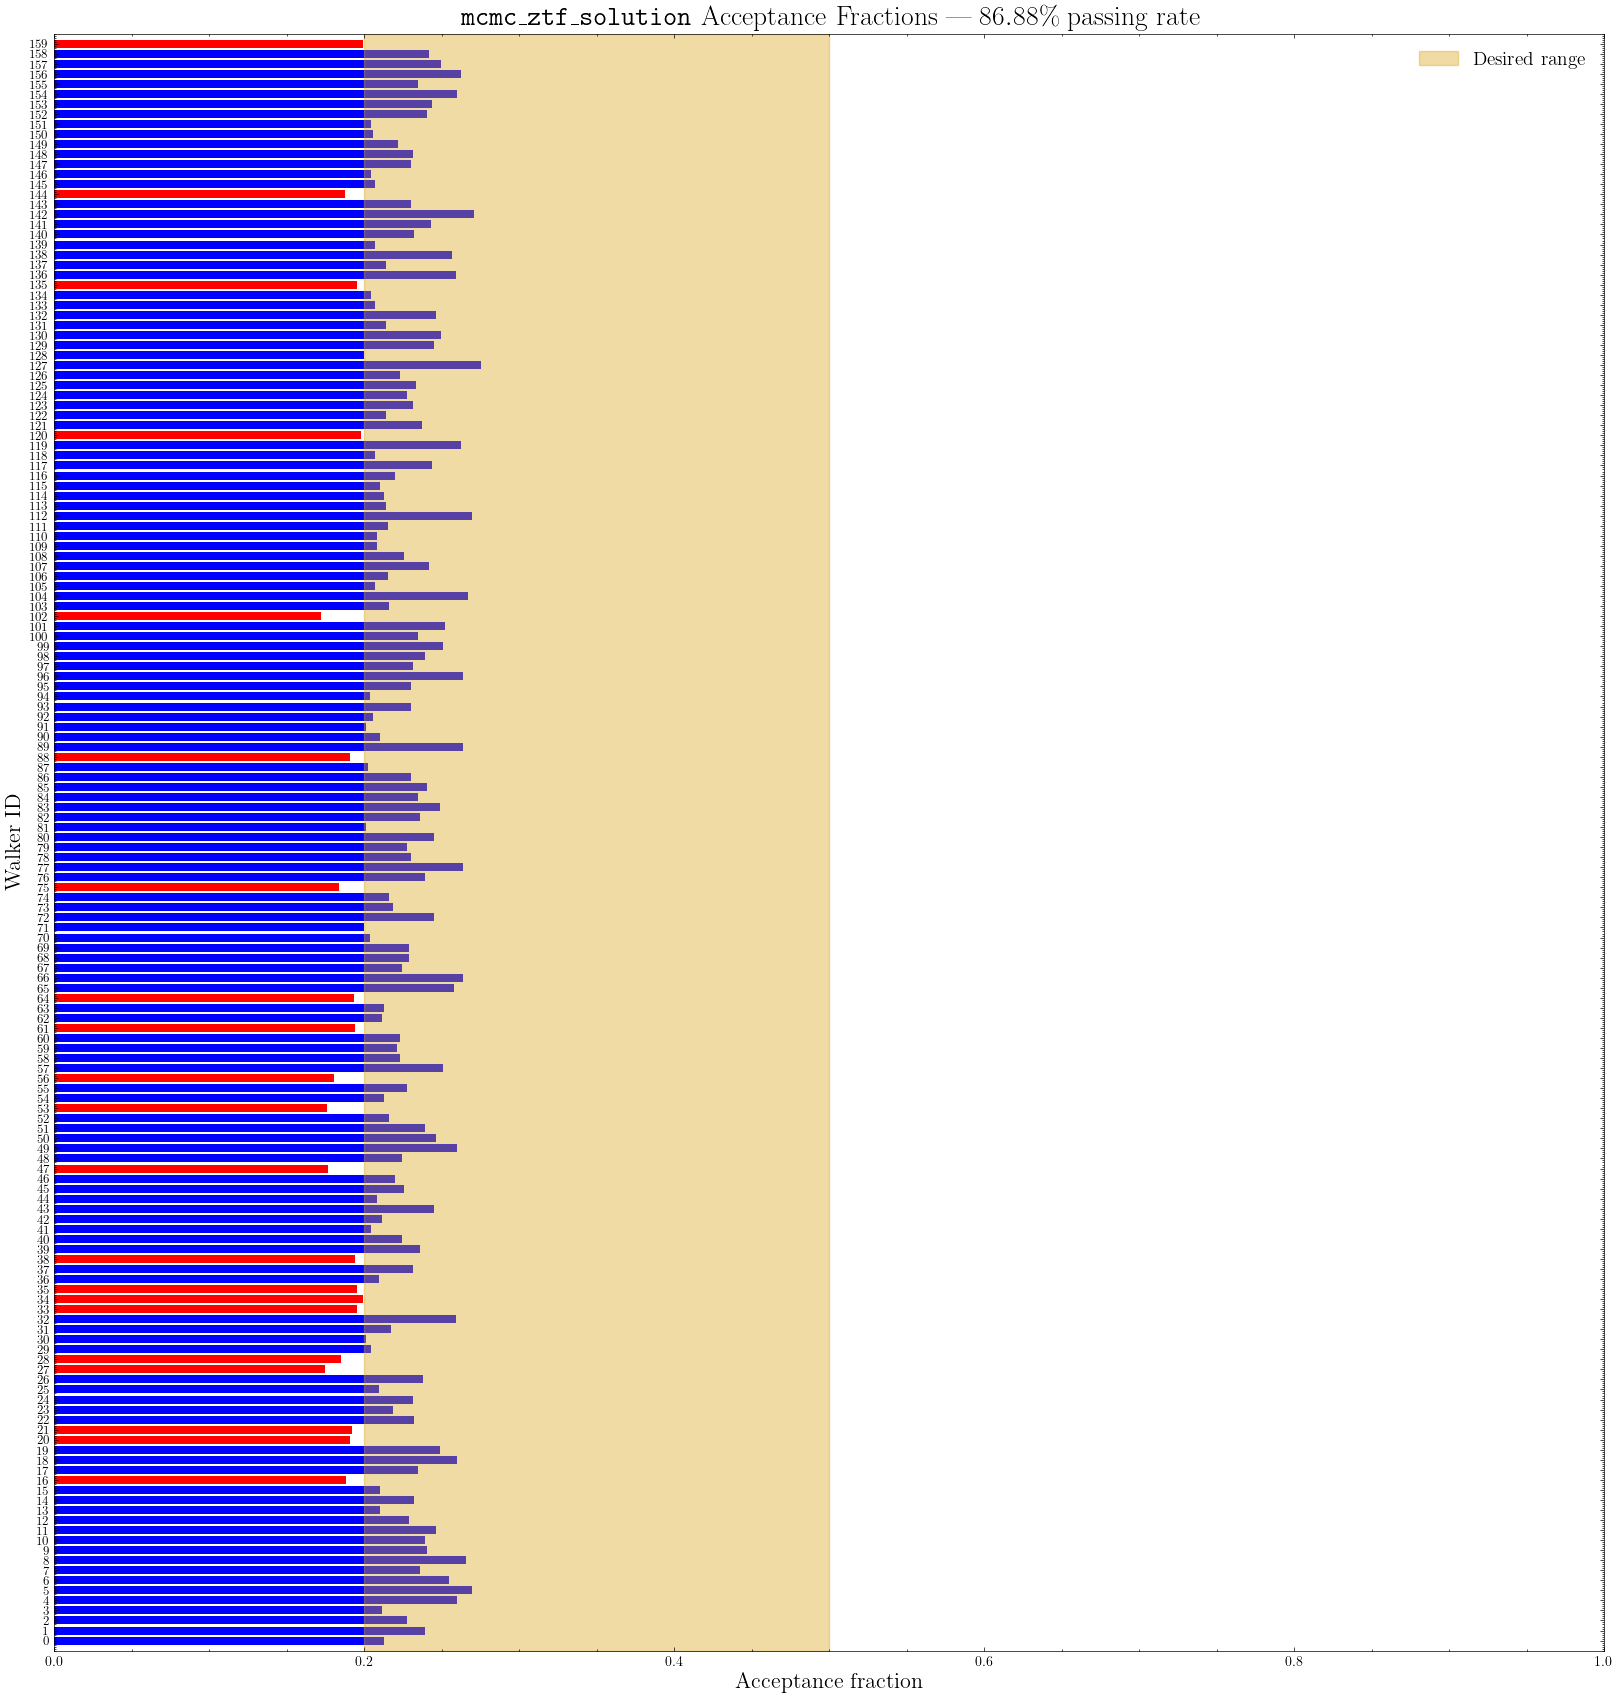
\includegraphics[scale=0.36]{Metodologia/Secciones/ModeloComputacional/Figures/Figura MCMC ZTF Acceptance Fractions.png}
	\caption{Fracción de pasos aceptados (eje \code{x}) para cada caminador (eje
	\code{y}) en el muestreo después de 865 iteraciones. El rango ideal de 0.2 a
	0.5 está marcado por la región amarilla. Aquellos caminadores que no estén
	dentro de este rango están resaltados por barras rojas.}
	\label{figuraFraccionPasosAceptados}
\end{figure}

\subsubsection{Errores en el Espacio de Parámetros}

Es inevitable que mientras los caminadores exploren el espacio de parámetros
encuentren una combinación de valores que resulten en un modelo inválido, ya sea
por limitaciones técnicas de PHOEBE o porque esa combinación en particular
resulta en un sistema físicamente imposible. Estos resultan en errores, y por
ende PHOEBE los trata como pasos fallidos. El resolvedor de tipo MCMC de PHOEBE
es capaz de mantener un registro de todas las muestras fallidas y mostrarlas en
una gráfica, para poder identificar fácilmente cualquier región de interés. En
la \reffigure{figuraMcmcMuestrasFallidas} se pueden ver las muestras
fallidas en la cadena de este modelo.

\begin{figure}[!ht]
	\centering
	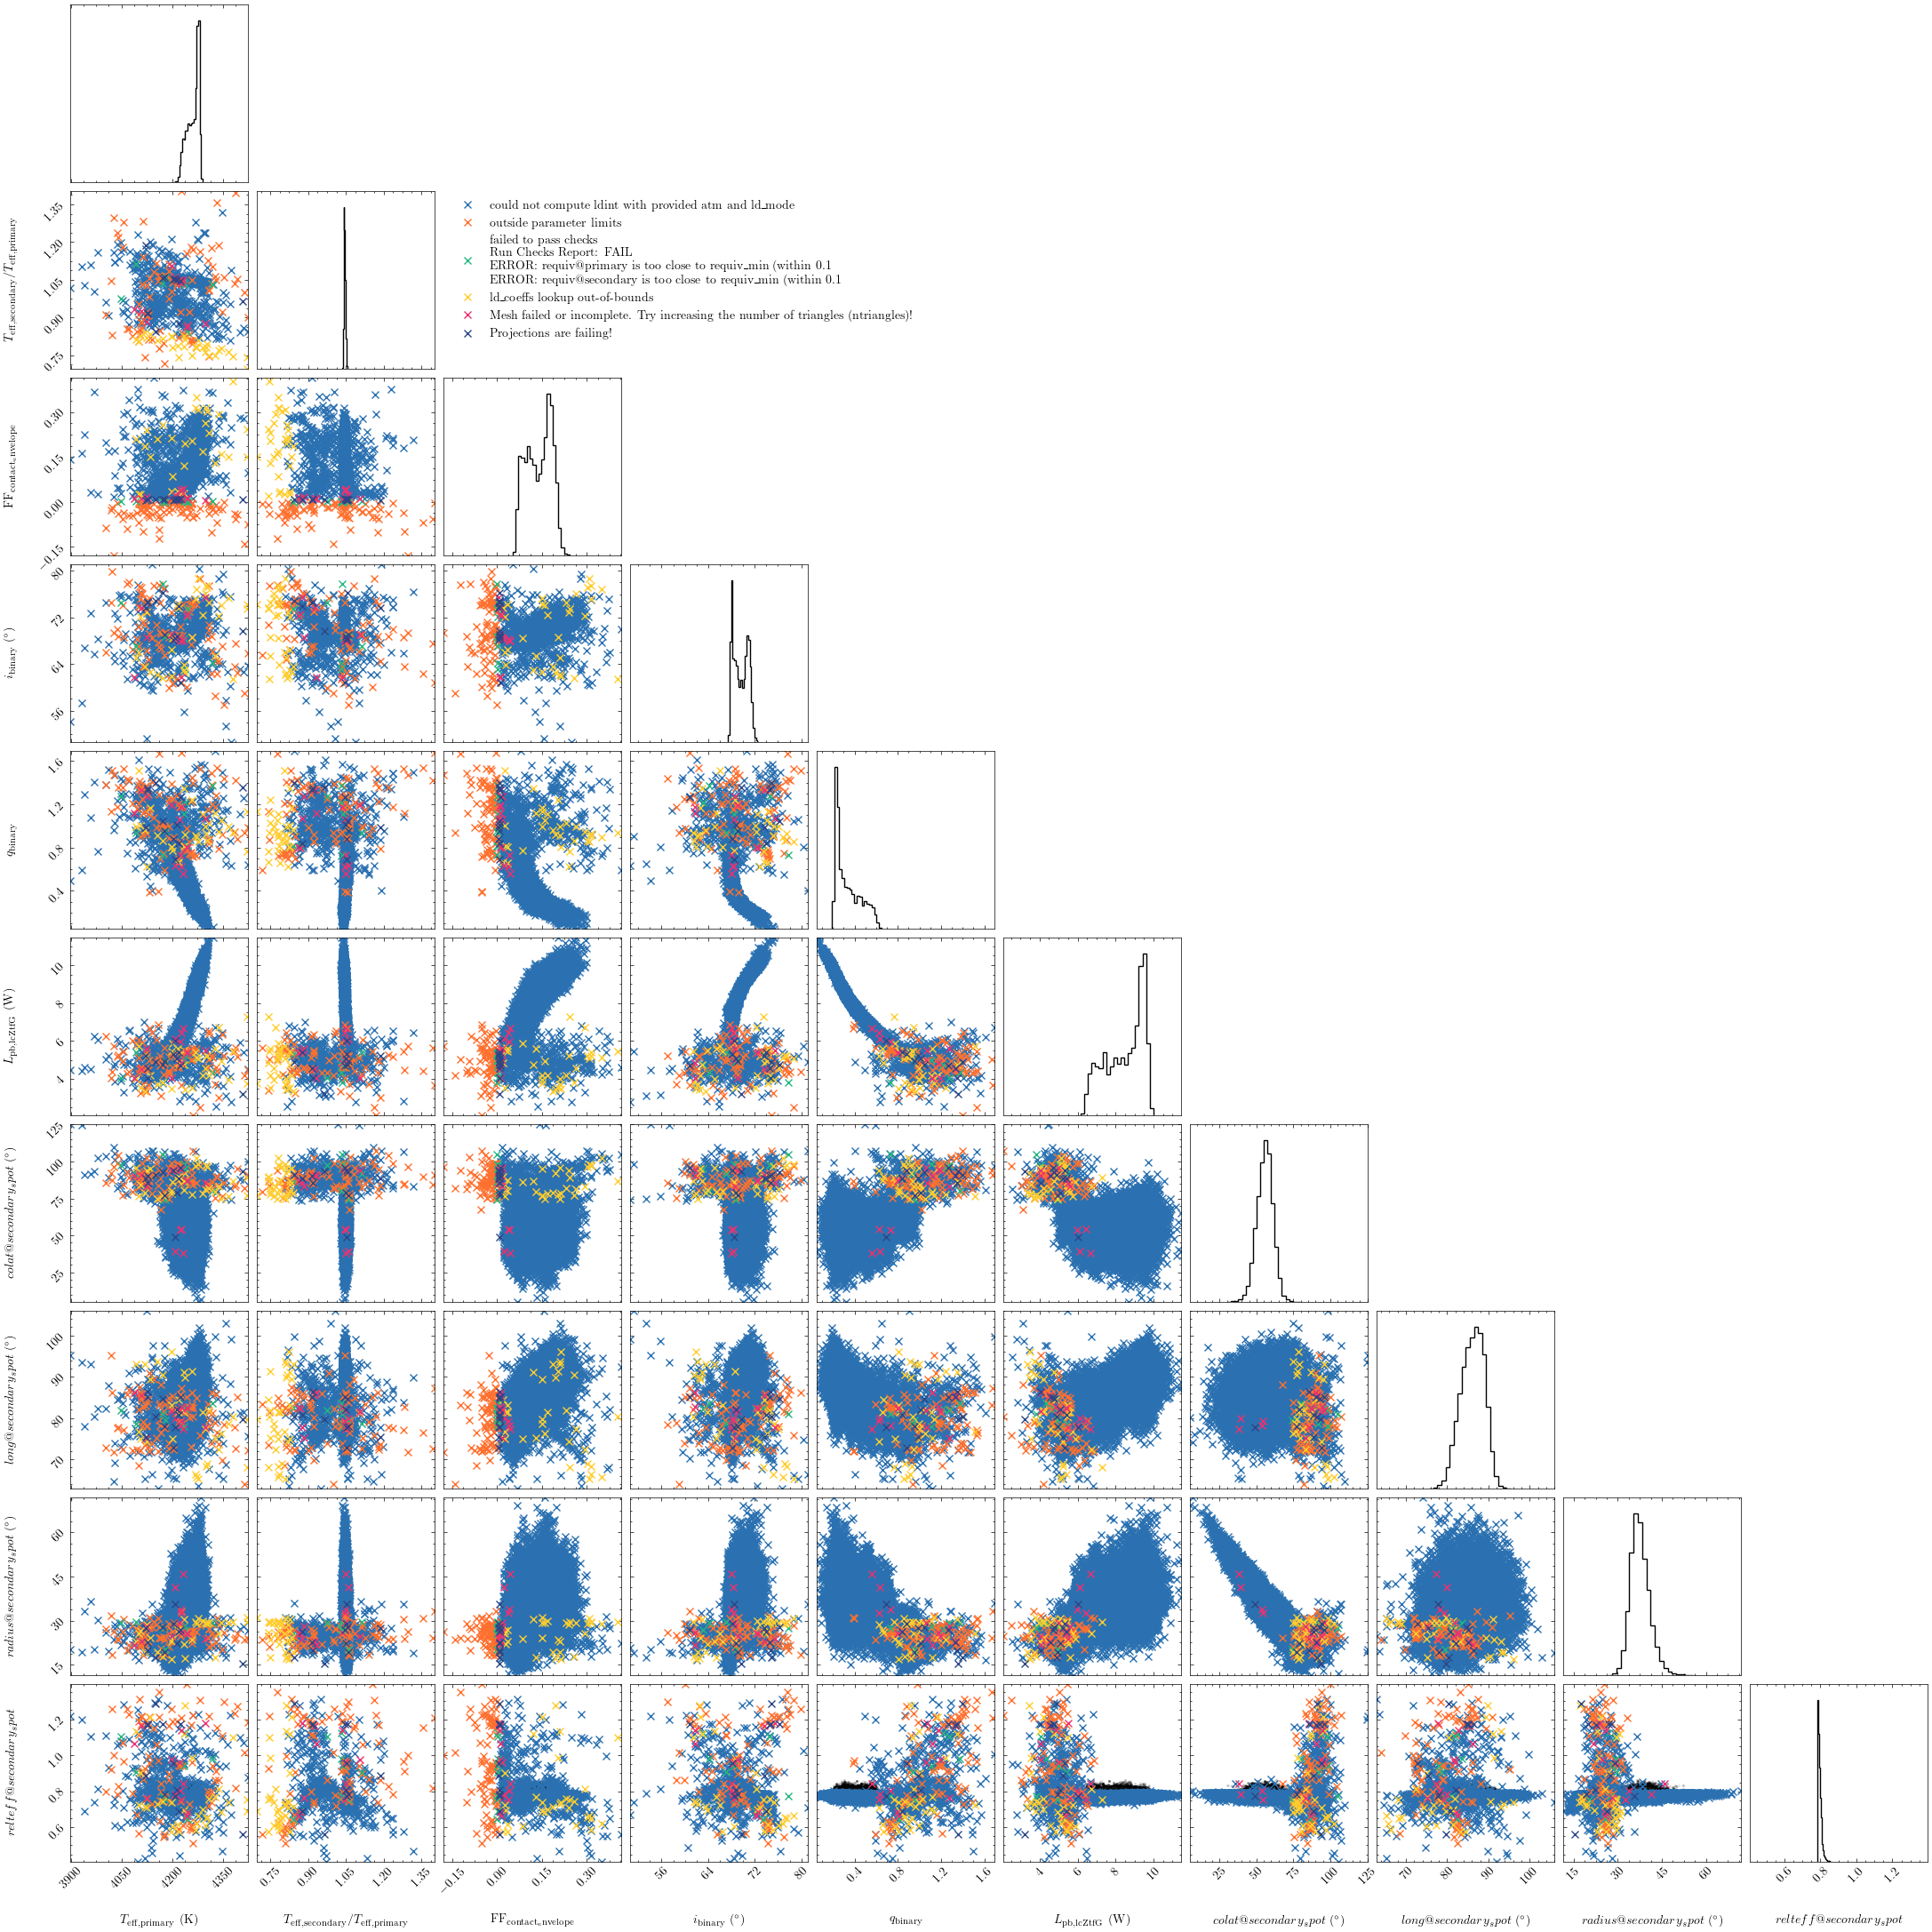
\includegraphics[scale=0.26]{Metodologia/Secciones/ModeloComputacional/Figures/Figura MCMC Failed.png}
	\caption{Muestras obtenidas del proceso MCMC que resultaron en una falla del modelo hacia adelante, después de 2870 iteraciones.}
	\label{figuraMcmcMuestrasFallidas}
\end{figure}

La gran mayoría de fallas en las muestras son consecuencia de valores inválidos
dado la atmósfera estelar de
\citeyearparen{castelli_kurucz_new_model_atmospheres_2004}, representados por
las marcas azules, específicamente con respecto al oscurecimiento al limbo. No
se modificó ningún parámetro para mitigar estos errores, principalmente debido a
que no muestran una frontera claramente definida. Las marcas de color azul
oscuras indican una falta de triángulos en la malla de la superficie estelar;
esto se mitigó aumentando el número de triángulos del modelo por medio del
parámetro \code{ntriangles} para permitir que los caminadores exploraran
regiones del espacio de parámetros que requieran una mayor resolución espacial,
como la frontera del factor de relleno $f = 0$. No se implementó alguna solución
para el resto de los errores debido a su baja cantidad, lo cual indica que no
son un problema significativo para seguir explorando el espacio de parámetros de
manera adecuada. 

\subsubsection{Camino Trazado por los Caminadores}

PHOEBE ofrece la posibilidad de ver el camino trazado por cada caminador
individual del muestreo. Una inspección visual nunca debería ser la única fuente
para una conclusión del modelo; sin embargo, es especialmente útil para
identificar problemas obvios con el muestreo, los cuales pueden ser analizados
sistemáticamente por medio de código u otros métodos reproducibles. Las gráficas
fueron producidas utilizando el argumento \code{style} dado a la función
\code{plot} del bundle de PHOEBE. Para identificar si el muestreo ha logrado
encontrar una solución óptima se acudió al trazo de los caminadores con respecto
a la probabilidad logarítmica (\code{lnprobability}) del modelo resultante, el
cual se puede ver en la \reffigure{figuraCaminadoresTrazoLnprobability}.

\begin{figure}[!ht]
	\centering
	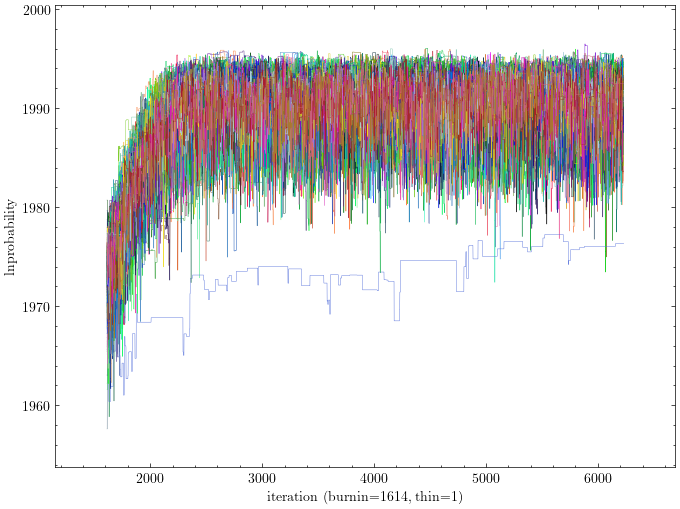
\includegraphics[scale=0.56]{Metodologia/Secciones/ModeloComputacional/Figures/Figura Caminadores Trazo lnprobability.png}
	\caption{La probabilidad logarítmica de cada uno de los 160 caminadores que
	forma la cadena de Markov después de 6233 iteraciones. Con la excepción de
	un individual, todos los caminadores llegaron a converger a un espacio de
	parámetros que son igual de válidos dados las curvas observacionales de
	ZTF.}
	\label{figuraCaminadoresTrazoLnprobability}
\end{figure}

También es posible ver tendencias en el vector de parámetros de cada caminador;
a simple vista es posible identificar tendencias en general si los caminadores
están migrando a una región en particular de cada parámetro, o si algún
caminador se ha quedado inmóvil, el cual también se podría reflejar en la
fracción de pasos aceptados. Esto se puede ver en la
\reffigure{figuraCaminadoresTrazoParametros}.

\begin{figure}[!ht]
	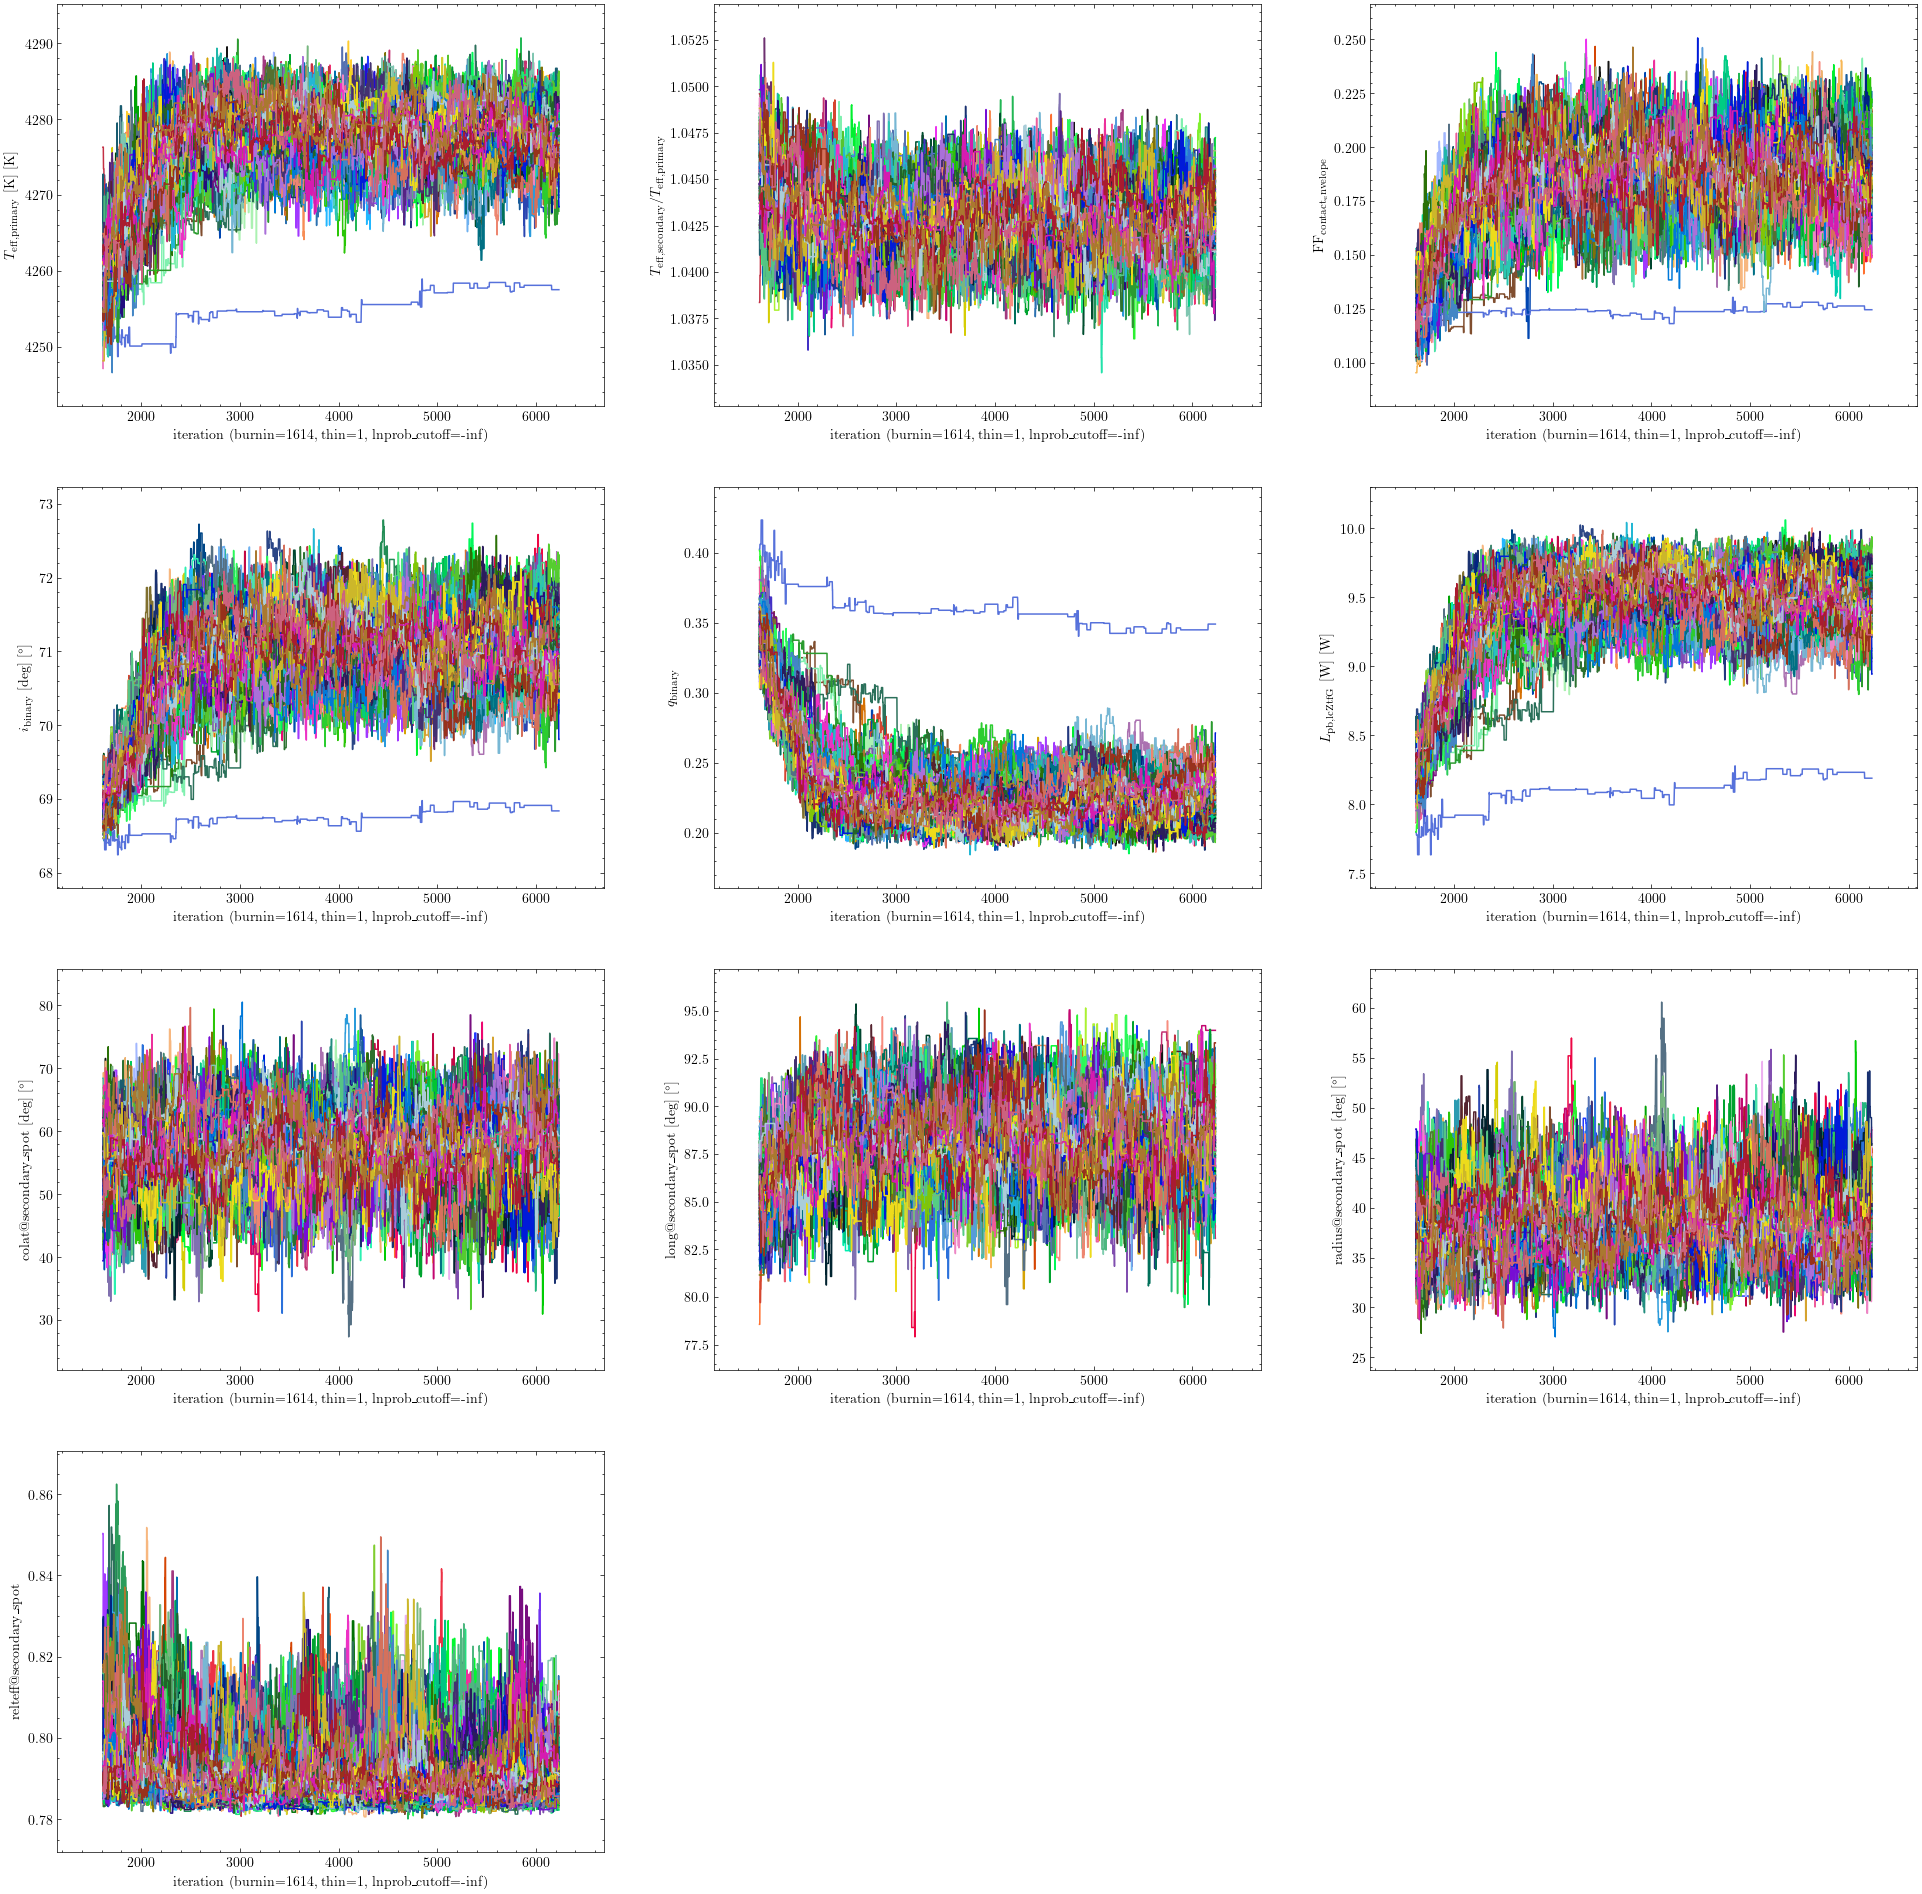
\includegraphics[scale=0.3]{Metodologia/Secciones/ModeloComputacional/Figures/Figura Caminadores Trazo Parametros.png}
	\caption{El valor de cada parámetro muestreado para cada caminador como
	función de iteraciones corridas del muestreo después de 6233 iteraciones. Se
	puede ver un punto alrededor de las 2200 iteraciones a partir de la cual los
	caminadores se establecen en una región bien definida para cada parámetro,
	lo cual es un indicador que el muestreo ha convergido.}
	\label{figuraCaminadoresTrazoParametros}
\end{figure}

Se ha especificado un tiempo de quemado de 1614 iteraciones para ambas gráficas,
eliminando todas las iteraciones previas. Para ver la ruta completa que han
tomado los caminadores con respecto a los parámetros del modelo se hace
referencia al apéndice en la
\refthesissection{apendice:modelo_computacional_graficas:trazos_completos_caminadores}
(las figuras de tamaño completo se pueden ver en el Notebook
\href{https://github.com/KnightIV/UANL_MAPTA_Observaciones/blob/main/analisis/phoebe_model/sampling/updated-data-mcmc-sampling.ipynb}{\code{updated-data-mcmc-sampling.ipynb}}).
En estas gráficas se puede apreciar el número de iteraciones que fueron
requeridas para llegar al espacio de parámetros más óptimo, lo cual resulta en
un muestreo ineficiente. Esto es una consecuencia de haber elegido una
distribución prior uniforme no informativa para el muestreo. El caso ideal
hubiera sido que esta solución se hubiera encontrado en el proceso de optimización;
la migración de los caminadores requirió una gran cantidad de iteraciones, y por
lo tanto un enorme tiempo de cómputo que efectivamente se tiene que utilizar
como periodo de quemado.

% TODO: actualiza con las últimas iteraciones
\section{Resultados} \label{metodologia:modelocomputacional:resultados}

Es prácticamente imposible determinar con certeza si una cadena de Markov ha
convergido con éxito a un volumen del espacio de parámetros para un modelo de un
sistema binario estelar. Esto se debe al alto número de dimensiones involucradas
en el modelo; esto corresponde a una disminución significativa en la fracción de
pasos aceptados, y por ende un aumento en el tiempo de autocorrelación
(\citeyearparen{speagle_conceptual_intro_mcmc_2020}). Por lo tanto, por
cuestiones de tiempo se detuvo el muestreo de MCMC llegando a las 6413
iteraciones, de las cuales 2200 se utilizaron de quemado antes de converger. Un
análisis visual de los trazos de los caminadores demuestra que todos los
caminadores llegaron a un espacio de parámetros bien definido, del cual no salen
en el resto del muestreo. El tiempo de autocorrelación promedio de todos los
parámetros fue de $647.14$, el cual corresponde a un promedio de $7.36$ muestras
independientes e idénticamente distribuidas (IIDs); la inclinación orbital fue
el parámetro peor muestreado, con un tiempo de autocorrelación de $826.86$
iteraciones, llegando a $5.76$ IIDs. En promedio la cadena mostró una fracción
de pasos aceptados de $0.04$. Esto es significativamente menos del rango
recomendado por \citeyearparen{foreman-mackey_emcee_2013} de 0.2 a 0.5, el cual
también es un síntoma de un modelo de alta dimensionalidad. El código
responsable por correr el muestreo se tuvo que reiniciar varias veces en el
transcurso del proyecto, lo cual al experimentar con el código tuvo un impacto
subjetivo en la fracción de pasos aceptados reportado por PHOEBE; antes del
primer reinicio el muestreo (4260 iteraciones, 1159 iteraciones de quemado.)
tenía una fracción de pasos aceptados promedio de $0.196$, con el 43.12\% de los
caminadores ostentando una fracción de pasos aceptados entre 0.2 y 0.5. 

% TODO: actualiza con últimos resultados
\subsection{Funciones de Densidad de Probabilidad a Posteriori} \label{metodologia:modelocomputacional:mcmc:resultados}

Las funciones de densidad de probabilidad (PDFs por sus siglas en inglés) se
pueden revisar tanto a lo largo del proceso utilizando los archivos de progreso,
como hasta el final que haya terminado de correr el número de iteraciones
configuradas en el resolvedor. Utilizando la distribución de las muestras en la
cadena se puede determinar las incertidumbres de cada parámetro y al mismo
tiempo inspeccionar de manera visual las correlaciones que existen entre
diferentes parámetros. La \reffigure{figuraMcmcZtfResultadosPrimarios} muestra
estas distribuciones.

% TODO: actualiza con últimos resultados y número iteraciones
\begin{figure}[!ht]
	\centering
	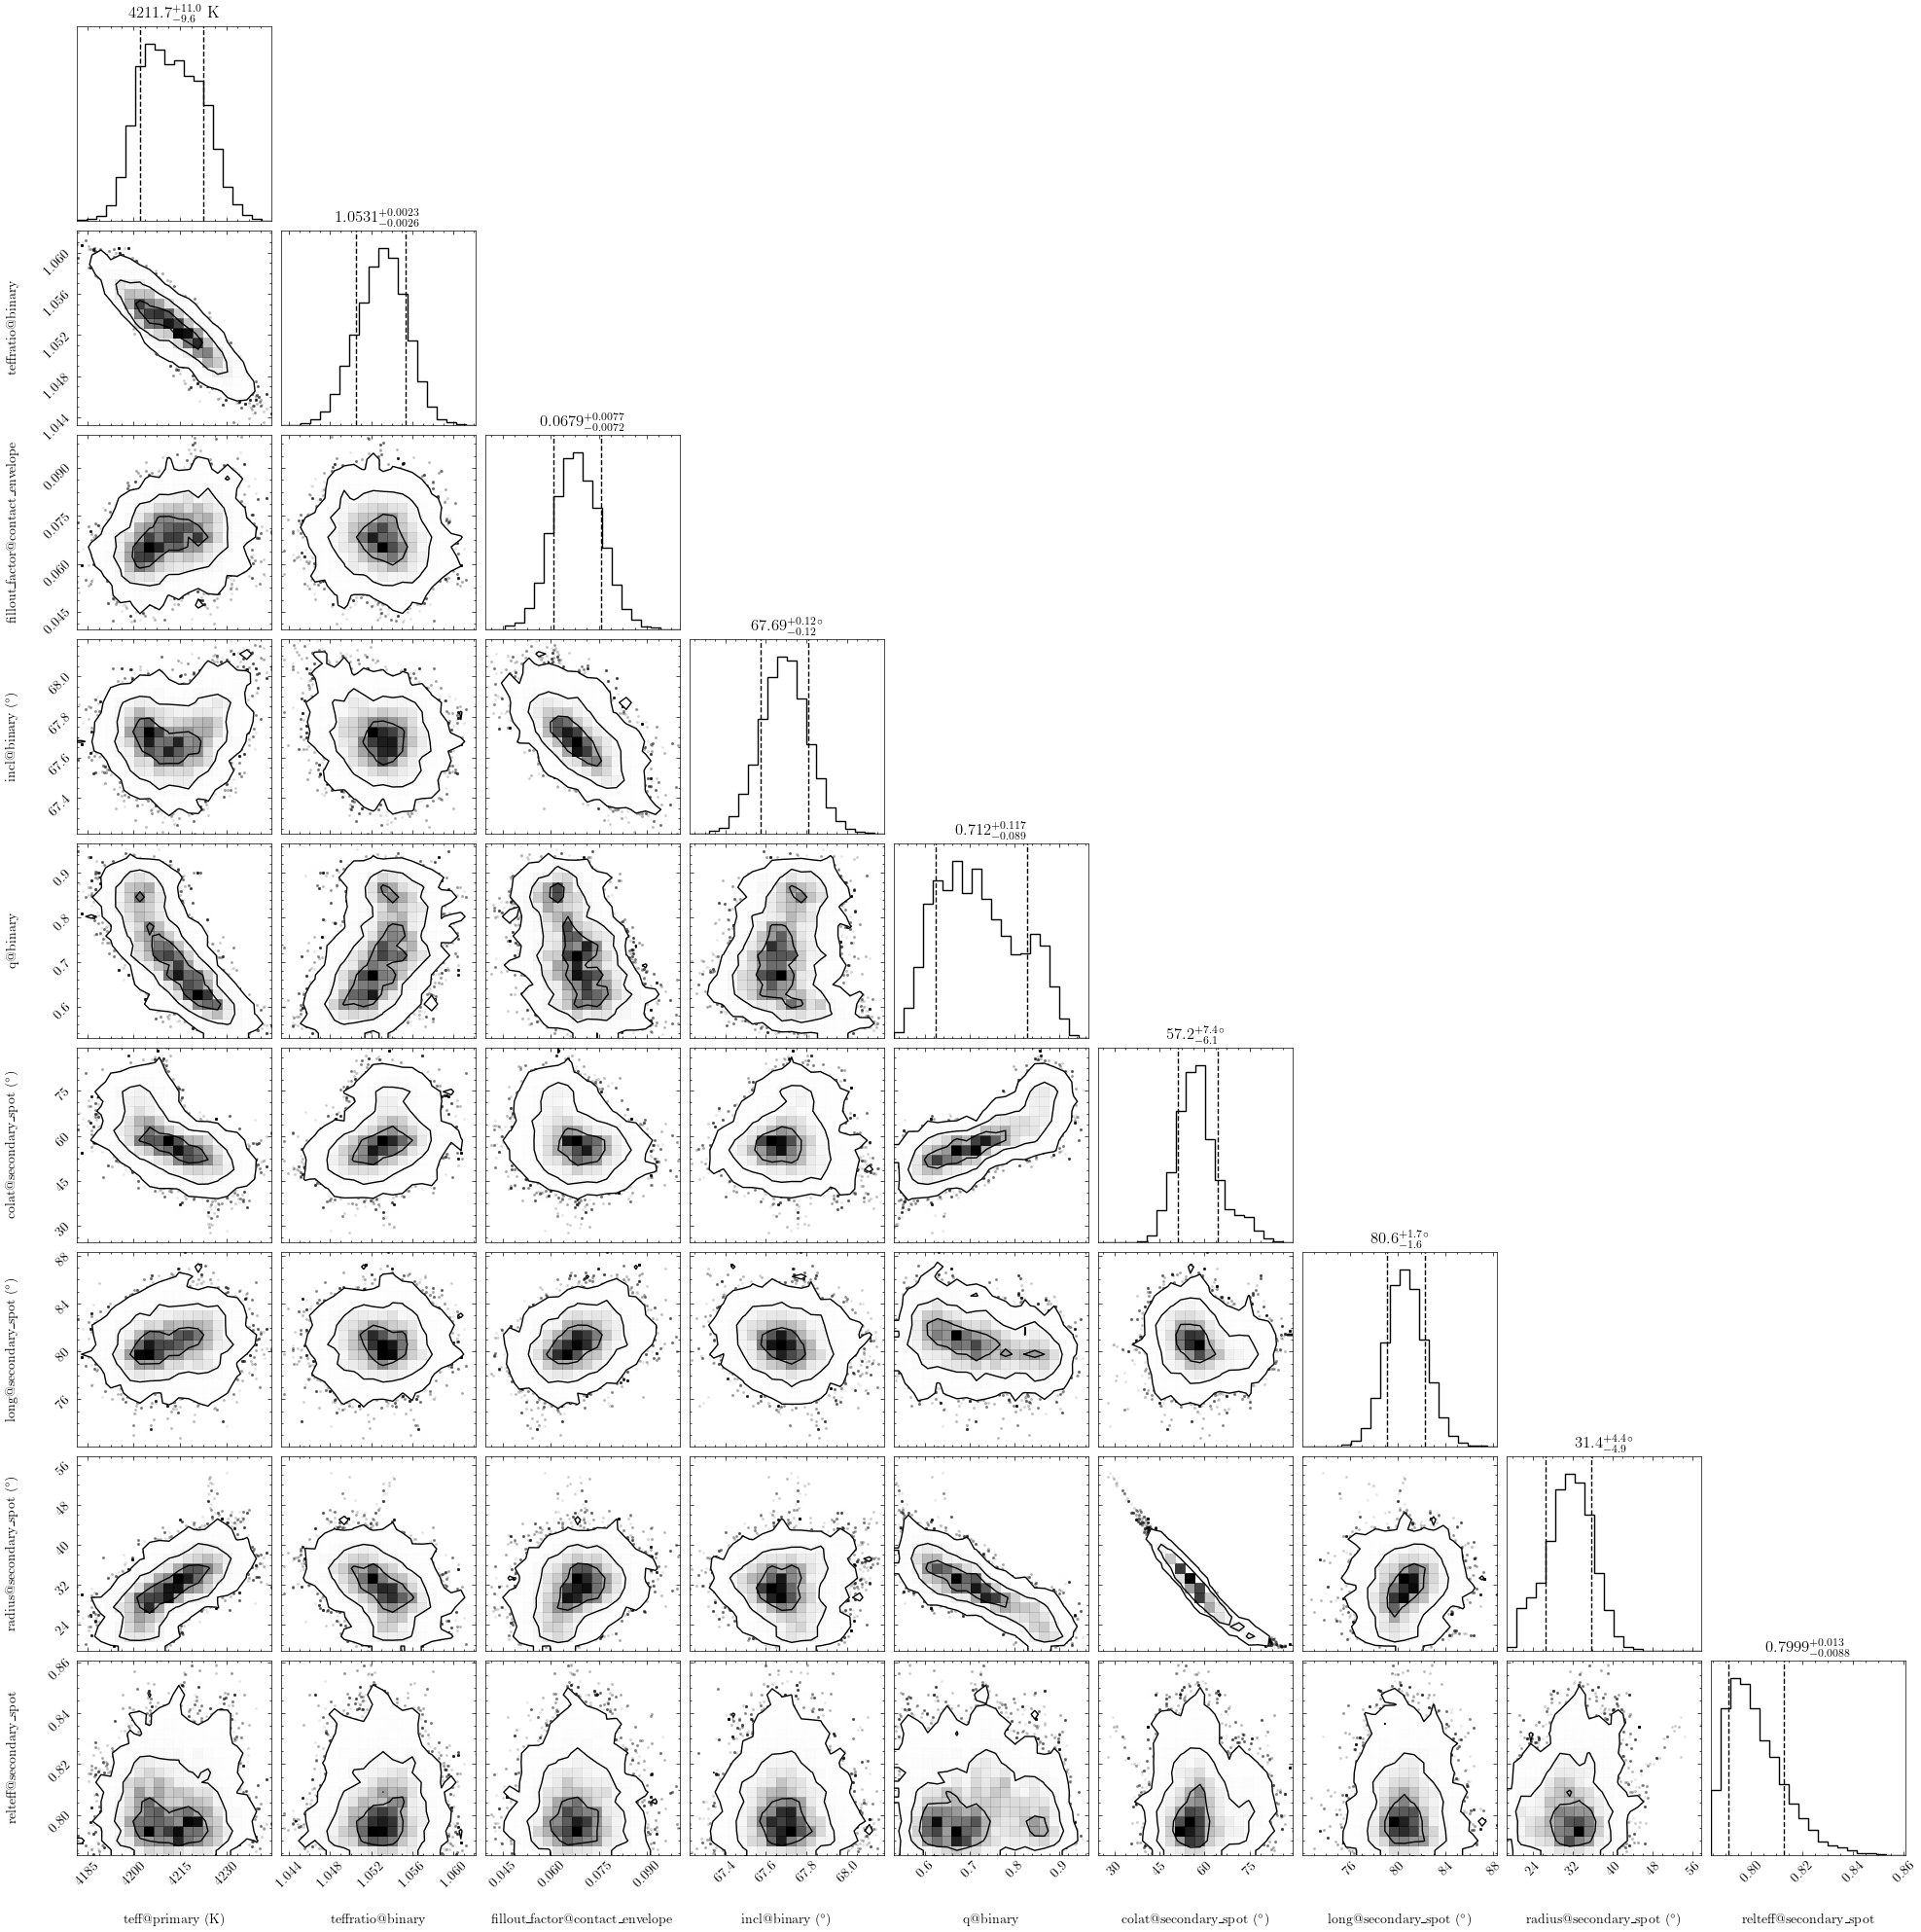
\includegraphics[scale=0.29]{Metodologia/Secciones/ModeloComputacional/Figures/Figura MCMC ZTF Resultados.png}
	\caption{Gráfica mostrando las muestras en la cadena después de 6413
	iteraciones (2200 iteraciones de tiempo de quemado), marginalizando sobre la
	luminosidad de el pasabanda ZTF:g en la muestra. Se aplicó un corte de
	calidad, aceptando solo las muestras cuya probabilidad logarítmica sea mayor
	a 1980 (utilizando el argumento $\mathtt{lnprob\_cutoff} = 1980$). La
	mayoría de los parámetros muestran una forma Gaussiana, de las cuales se
	obtiene los valores promedio junto a sus incertidumbres. La temperatura
	relativa de la mancha estelar \code{relteff} muestra una forma Gaussiana
	sesgada.}
	\label{figuraMcmcZtfResultadosPrimarios}
\end{figure}

La luminosidad se incluyó como un parámetro de molestia, el cual afecta el
modelo sintético resultante, pero no es un parámetro que nos interese medir.
Para los parámetros de interés se marginaliza (integra) sobre todos los
parámetros de molestia, incluyéndolos como parámetros que muestrear. La figura
completa incluyendo la luminosidad de pasabanda de ZTF:g se puede ver en el
apéndice en la \reffigure{figuraPhoebeMcmcResultadosCompletos}. Todas las
distribuciones posteriores en la cadena muestran una forma asimétrica, algunas
más pronunciadas que otras. PHOEBE reporta el valor promedio obtenido en la
muestra y 2 intervalos de confianza, los cuales se reportan en la
\reftable{tablaMcmcResultadosIncertidumbres}.

% TODO: actualiza con últimos resultados y número de iteraciones
{\renewcommand{\arraystretch}{1.5}%
\begin{table}[!ht]
	\centering
	\begin{tabular}{|P{3cm}|P{4cm}|}
		\hline
		\thead{Parámetro}                        & \thead{Valor} \\
		\hline
		$T_1$ & $4278.3^{ +3.1 }_{ -3.5 } ~\mathrm{K}$ \\
		\hline
		$T_2 / T_1$ & $1.0428^{ +0.0015 }_{ -0.0015 } \mathrm{}$ \\
		\hline
		$f$ & $0.187^{ +0.015 }_{ -0.015 } \mathrm{}$ \\
		\hline
		$i_\mathrm{orb}$ & $71.06^{ +0.4 }_{ -0.43 } \mathrm{{}^{\circ}}$ \\
		\hline
		$q$ & $0.223^{ +0.014 }_{ -0.011 } \mathrm{}$ \\
		\hline
		$\mathrm{ L_\mathrm{ pb, ZTF:g } }$ & $9.52^{ +0.14 }_{ -0.18 } ~\mathrm{W}$ \\
		\hline
		$\mathrm{Lat}_{\mathrm{spot}}$ & $58.2^{ +4.8 }_{ -5.3 } \mathrm{{}^{\circ}}$ \\
		\hline
		$\mathrm{ Lon }_{\mathrm{spot}}$ & $88.3^{ +1.8 }_{ -1.8 } \mathrm{{}^{\circ}}$ \\
		\hline
		$\mathrm{ Radius }_{\mathrm{spot}}$ & $37.9^{ +3.4 }_{ -2.7 } \mathrm{{}^{\circ}}$ \\
		\hline
		$T_{\mathrm{spot}} / T_2$ & $0.7893^{ +0.0073 }_{ -0.0038 } \mathrm{}$ \\
		\hline
	\end{tabular}
	\caption{Valores obtenidos de la cadena de Markov junto a sus incertidumbres
	asimétricas. Estos valores fueron calculados después de 6233 iteraciones.}
	\label{tablaMcmcResultadosIncertidumbres}
\end{table}}

\subsection{Incertidumbres en el Modelo Hacia Adelante}

Utilizando las distribuciones posteriores es posible visualizar la dispersión en
el modelo sintético. Esto se hace con el parámetro \code{sample\_from} del
cómputo en uso, en el cual se pueden especificar las distribuciones de las cuales
obtener muestras individuales, calculando un modelo hacia adelante a partir de las
distribuciones obtenidas. En la \reffigure{figuraMcmcZtfModeloDispersionPosterior} se
puede apreciar la dispersión (en las regions oscurecidas) del modelo promedio,
el cual surge como resultado de las incertidumbres de cada parámetro. Este
cálculo requiere de una gran cantidad de memoria para poder generar un alto
número de muestras, por lo cual se disminuyó el número de muestras de 50 a 25;
aún con relativamente pocas muestras se puede apreciar como el modelo promedio
se ajusta a los datos observacionales. Al calcular la probabilidad logarítmica
del modelo vemos que el muestreo llegó a un espacio de parámetros que mejor
explican las curvas observadas, obteniendo una puntuación de $1844.72$ contra
$1688.85$ del último modelo optimizado de la
\refthesissection{metodologia:modelocomputacional:optimizacion}.

% TODO: actualiza cuando corran más iteraciones
\begin{figure}[!ht]
	\centering
	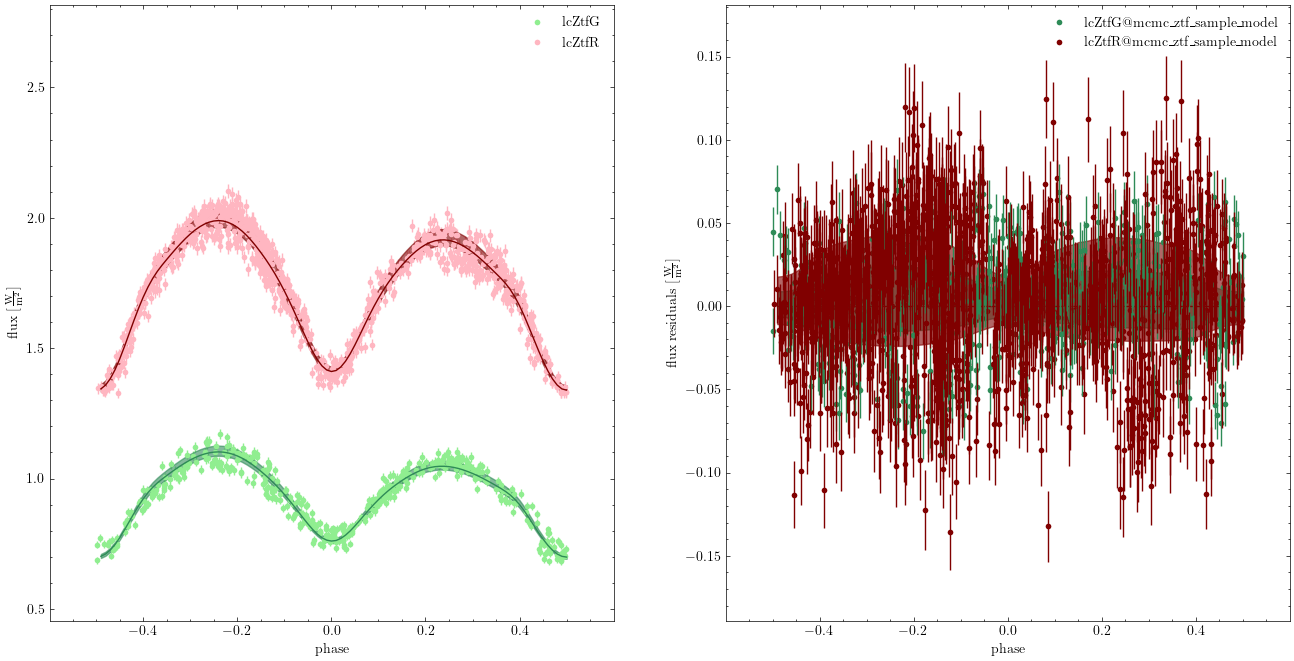
\includegraphics[scale=0.45]{Metodologia/Secciones/ModeloComputacional/Figures/Figura MCMC ZTF Modelo.png}
	\caption{Modelo sintético generado por PHOEBE utilizando muestras de la
	estimación de la distribución posterior obtenida mediante el proceso MCMC.
	Este modelo fue calculado con 25 muestras en total de las distribuciones
	posteriores.}
	\label{figuraMcmcZtfModeloDispersionPosterior}
\end{figure}

\begin{figure}[!ht]
	\centering
	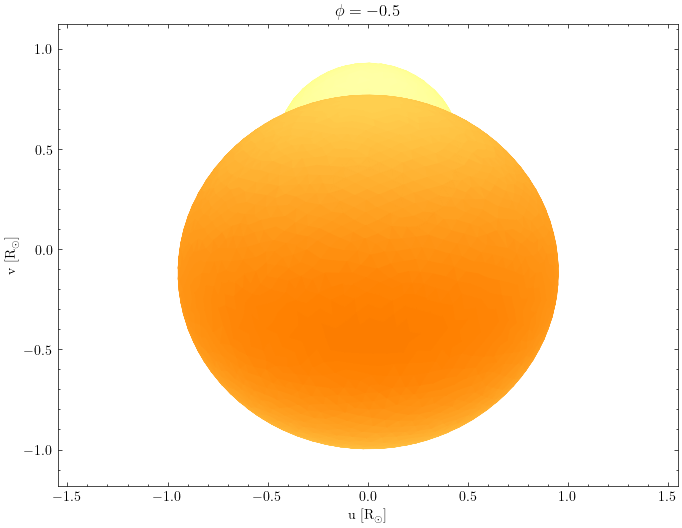
\includegraphics[width=0.49\linewidth]{Metodologia/Secciones/ModeloComputacional/Figures/Figura MCMC Mesh Modelo -0.5.png}
	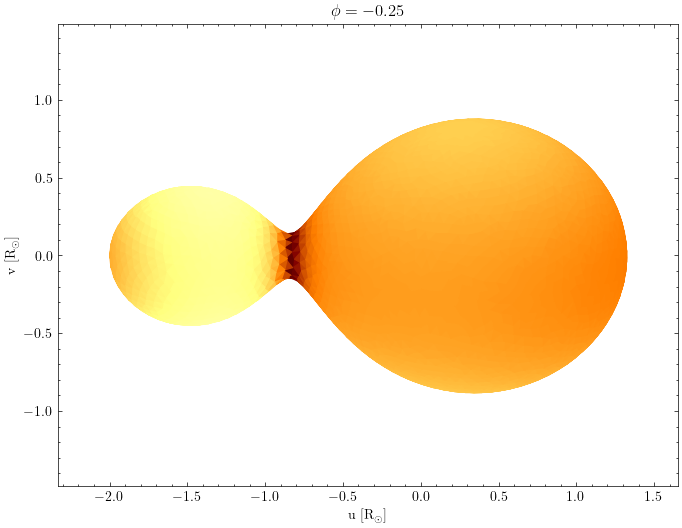
\includegraphics[width=0.49\linewidth]{Metodologia/Secciones/ModeloComputacional/Figures/Figura MCMC Mesh Modelo -0.25.png}
	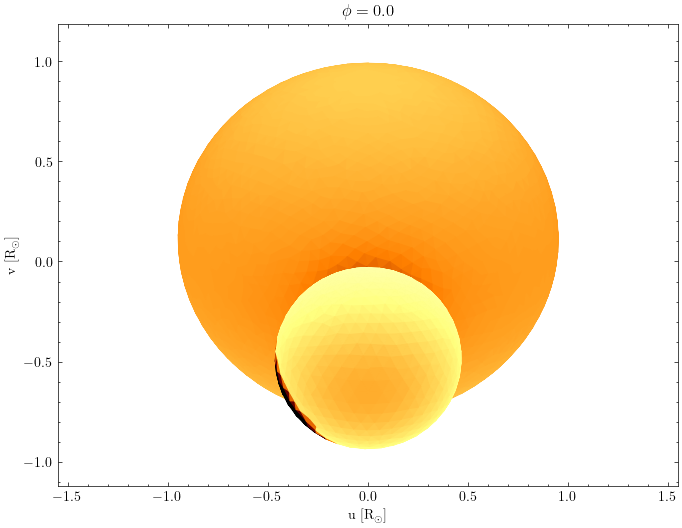
\includegraphics[width=0.49\linewidth]{Metodologia/Secciones/ModeloComputacional/Figures/Figura MCMC Mesh Modelo 0.png}
	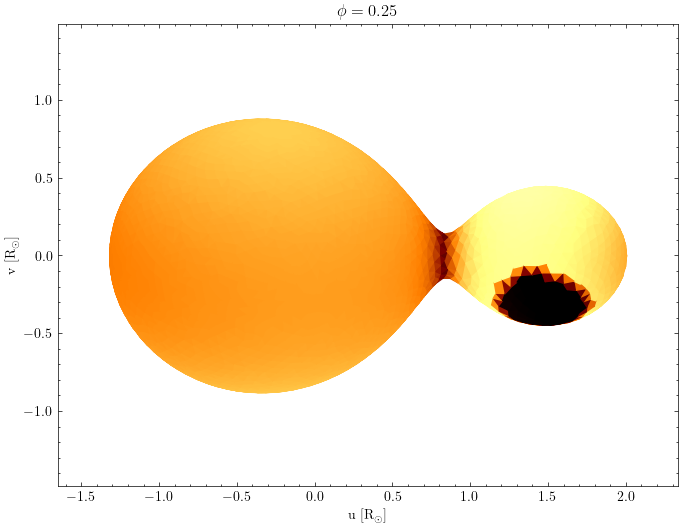
\includegraphics[width=0.49\linewidth]{Metodologia/Secciones/ModeloComputacional/Figures/Figura MCMC Mesh Modelo 0.25.png}
	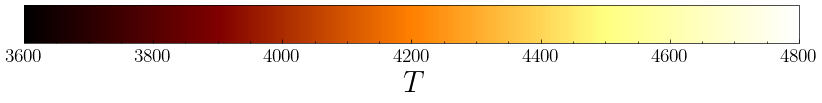
\includegraphics[width=1\linewidth]{Metodologia/Secciones/ModeloComputacional/Figures/Figura MCMC Mesh Modelo Colorbar.png}
	\caption{Malla del modelo sintético generado utilizando los valores
	promedios de los PDFs resultados. El color de cada elemento superficial
	representa la temperatura efectiva local; se logra apreciar la mancha
	estelar fría presente en la componente secundaria.}
\end{figure}